\documentclass[11pt,letterpaper]{article}
\usepackage{fontspec}
\setmainfont{texgyrepagella}[Extension=.otf,UprightFont=*-regular,BoldFont=*-bold,ItalicFont=*-italic,BoldItalicFont=*-bolditalic]
\usepackage[bidi=default]{babel}
\babelprovide[import,main]{spanish}
\babelprovide[import]{hebrew}
\babelprovide[import]{ancientgreek}
\babelfont[hebrew]{rm}[Path=fonts/,BoldFont=NotoHebrewSerif-700.ttf,Scale=0.95]{NotoHebrewSerif-400.ttf}
\babelfont[ancientgreek]{rm}[Path=fonts/]{GFSPorson.otf}
\newcommand{\heb}[1]{\mbox{\foreignlanguage{hebrew}{#1}}}
\newcommand{\grc}[1]{\foreignlanguage{ancientgreek}{#1}}
\newcommand{\hebverso}[1]{\par\smallskip{\centering\begin{otherlanguage}{hebrew}\large #1\end{otherlanguage}\par}\smallskip}
\newcommand{\SENOR}{\textsc{Señor}}
\usepackage[margin=2.5cm,headheight=14pt]{geometry}
\usepackage{microtype,ragged2e,booktabs,graphicx,xcolor,csquotes,array}
\usepackage[hidelinks]{hyperref}\usepackage{xurl}\urlstyle{same}
\usepackage[most]{tcolorbox}
\usepackage{tikz}\usetikzlibrary{arrows.meta,positioning,calc,decorations.pathreplacing,shapes.geometric}
\usepackage{titlesec,fancyhdr,needspace,etoolbox}
\pretocmd{\section}{\needspace{6\baselineskip}}{}{}\pretocmd{\subsection}{\needspace{4\baselineskip}}{}{}
\definecolor{tierraroja}{RGB}{122,40,18}\definecolor{caferojizo}{RGB}{58,18,8}
\definecolor{mostaza}{RGB}{214,160,58}\definecolor{papiro}{RGB}{243,228,192}\definecolor{sepia}{RGB}{98,66,44}
\definecolor{oliva}{RGB}{92,98,48}
\titleformat{\section}{\Large\bfseries\color{tierraroja}}{\thesection.}{0.6em}{}
\titleformat{\subsection}{\large\bfseries\color{caferojizo}}{\thesubsection}{0.6em}{}
\pagestyle{fancy}\fancyhf{}
\fancyhead[L]{\foreignlanguage{spanish}{\small\itshape\color{sepia}Primicias}}\fancyhead[R]{\foreignlanguage{spanish}{\small\color{sepia}\thepage}}
\renewcommand{\headrulewidth}{0.4pt}
\setlength{\parindent}{1.27cm}\linespread{1.15}\setlength{\emergencystretch}{3em}
\newtcolorbox{cita}[1][]{enhanced,unbreakable,colback=tierraroja!5!white,colframe=tierraroja,boxrule=0pt,leftrule=2.5pt,arc=0pt,
  left=8pt,right=8pt,top=5pt,bottom=5pt,before skip=8pt,after skip=8pt,fontupper=\itshape,#1}
\newcommand{\fuente}[1]{\par\hfill{\upshape\bfseries\small\textcolor{tierraroja}{#1}}}
\newtcolorbox{nota}[1][]{enhanced,unbreakable,colback=mostaza!10,colframe=mostaza!85!tierraroja,boxrule=0.6pt,arc=2pt,
  fonttitle=\bfseries\small,coltitle=caferojizo,colbacktitle=mostaza!30,fontupper=\small,title={#1}}
\newtcolorbox{filologia}[1][]{enhanced,unbreakable,colback=white,colframe=tierraroja!45,boxrule=0.5pt,arc=2pt,
  fonttitle=\bfseries\small,coltitle=white,colbacktitle=tierraroja!80,fontupper=\small,title={Filología: #1}}
\newcommand{\refapa}[1]{\par{\RaggedRight\hangindent=1.27cm\hangafter=1\noindent #1\par}\vspace{4pt}}
\newcommand{\destacar}[1]{\textbf{\textcolor{tierraroja}{#1}}}
\newcolumntype{L}[1]{>{\RaggedRight\arraybackslash}p{#1}}

\title{\color{tierraroja}\bfseries Reshit y Bikurim: el Ómer de las primicias\\[4pt]\large\color{sepia}\mdseries ``Primicias de los que durmieron'' (1~Co 15:20)}
\author{}\date{}
\begin{document}
\maketitle\thispagestyle{empty}

\begin{abstract}\noindent
Entre la Pascua y Pentecostés, Levítico 23 ordena un rito breve que no es día de reposo ni convocación santa. El sacerdote mece ``delante del \SENOR'' la primera gavilla de la siega, el \emph{ómer reshit qetsirjem} (Lv 23:10--11), y desde ese día se cuentan cincuenta días hasta los dos panes de Shavuot. El capítulo estudia el rito con el método de la serie: histórico (la siega de la cebada en el mes de Abib, Gilgal, las primicias en Ezequías y Nehemías, la ceremonia del Segundo Templo según Josefo, Filón y la Misná), filológico (\emph{reshit}, \emph{bikurim}, \emph{terumá}, \emph{ómer}, \emph{tenufá}, \emph{lirtsonjem}; la Septuaginta \emph{drágma} y \emph{aparjé}; \emph{aparjé} y \emph{prōtótokos} en el Nuevo Testamento), textual (el debate sobre ``el día siguiente del sábado'' entre fariseos, saduceos y Qumrán, con sus consecuencias para Shavuot, y las variantes de 2~Ts 2:13, Ro 16:5 y Lc 6:1) y literario (Lv 23:9 abre una unidad que une la gavilla con Pentecostés; el patrón ``lo primero para Dios'' que corre desde Abel). Se expone la lectura del documento de referencia de la serie: Israel, libre del faraón tras cruzar el mar, es la primicia de las naciones (Éx 19:5--6; cf. Jer 2:3), y el Ómer representa al Señor Jesús recibido a la diestra del Padre; cumplido su objetivo, el rito dejó de tener vigencia. Se integra mi lectura anterior (el 17 de Nisán como día de las primicias y ``Jesús, primicia de la cosecha de cebada'') y se fija la cronología de la serie: crucifixión el 14 de Abib, resurrección al cerrarse el sábado 17 (``tres días y tres noches'', Mt 12:40) y presentación de Cristo como primicia el domingo 18, ``el día siguiente del sábado'', la misma fecha que el documento da a Israel; las cronologías tradicional y farisea quedan expuestas como alternativas, con las precisiones de cómputo correspondientes. La síntesis lee 1~Co 15:20--28 como el centro del tema: Cristo, las primicias; luego los de Cristo, en su venida; luego el fin.
\par\smallskip\noindent\textbf{Palabras clave:} primicias, \emph{ómer}, \emph{reshit}, \emph{bikurim}, \emph{tenufá}, Levítico 23, \emph{mimojorat hashabat}, \emph{aparjé}, 1~Corintios 15.\end{abstract}

\begin{nota}[Nota sobre el texto]
Las citas bíblicas son de la Reina-Valera 1960 (RVR1960), convención vigente de la serie. Donde esta escribe ``Jehová'', aquí se escribe \SENOR, que traduce el tetragrama \heb{יהוה}. Cuando la cita es traducción propia o paráfrasis, se indica. El hebreo sigue la \emph{Biblia Hebraica Stuttgartensia}; el griego, NA28 y la Septuaginta de Rahlfs-Hanhart. La Misná, el Talmud y los targumes se citan como \emph{tradición} (fuentes posteriores al Nuevo Testamento, aunque conserven prácticas antiguas). Los conteos de palabras se hicieron con la morfología del Códice de Leningrado (WLC) y del griego SBLGNT y Westcott-Hort incluidos en el repositorio Primera Línea; la redacción de la RVR1960 se cotejó con ediciones en línea. Todo lo que es lectura tipológica, cálculo cronológico o hipótesis se marca como precisión. El marco de la serie es su documento de referencia (lecciones 7, 8 y 11).
\end{nota}

%===================================================================
\section{Introducción: una gavilla antes de la siega}

Hay una ceremonia en Levítico 23 que no tiene fecha numérica, no es ``santa convocación'' y no prohíbe el trabajo. Dura lo que tarda un sacerdote en levantar y mover una gavilla de cebada delante del altar, y sin embargo de ella depende todo el calendario de la primavera: nadie en Israel podía comer pan del grano nuevo hasta ese día (Lv 23:14), y desde ese día se contaban las siete semanas que llevaban a Pentecostés (Lv 23:15--16). De ahí la pregunta que guía este estudio: \destacar{¿por qué la primera gavilla debía ir a Dios antes que a la mesa del agricultor?} El Nuevo Testamento obliga a añadir otra: ¿por qué Pablo, para explicar la resurrección, eligió precisamente esta palabra, ``Cristo, primicias de los que durmieron'' (1~Co 15:20)?

Sostengo en este capítulo que el Ómer condensa una ley que atraviesa toda la Escritura: \destacar{lo primero pertenece a Dios, y al entregarlo se consagra el resto}. Israel aprendió esa ley en el campo (la gavilla), en la familia (el primogénito) y en su propia historia (``Santo era Israel a \SENOR, primicias de sus nuevos frutos'', Jer 2:3); el Nuevo Testamento la aplica a Cristo resucitado, a la iglesia y a la cosecha final. La serie lee el rito como memorial de Israel, primicia de las naciones, y como figura de Cristo recibido a la diestra del Padre. El capítulo expone esa lectura y la contrasta con el texto, la historia y la tradición.

El recorrido es el habitual en la serie: el texto y sus paralelos legislativos (§2); las lecturas histórica (§3), filológica (§4), textual (§5) y literaria (§6); la lectura de la serie (§7); la fiesta en Jesús y los apóstoles (§8) y en la tradición judía (§9); la discusión de interpretaciones (§10), la síntesis (§11) y las preguntas para la reflexión (§12). En el ciclo de Levítico 23 el Ómer es la tercera ``estación'' de la primavera, entre los Ázimos y Shavuot.

\begin{center}
% === Esquema estándar de la serie: el ciclo de Levítico 23 ===
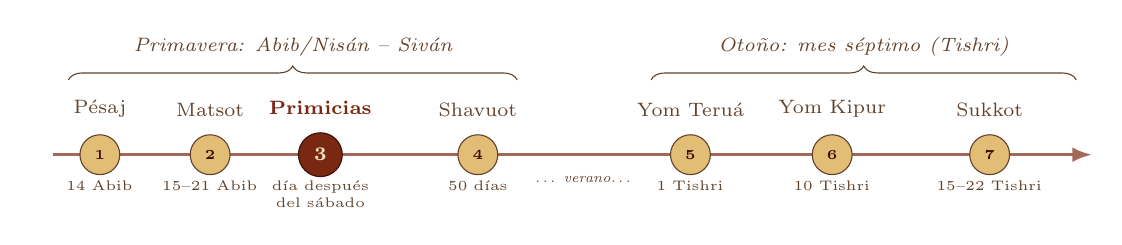
\begin{tikzpicture}[x=1cm,y=1cm,font=\scriptsize]
\def\fiestaactual{3}
 \draw[line width=1.2pt,tierraroja!70,-{Latex[length=2.5mm]}] (0,0) -- (13.2,0);
 \draw[decorate,decoration={brace,amplitude=5pt},sepia] (0.2,0.95) -- (5.9,0.95) node[midway,above=5pt,font=\scriptsize\itshape]{Primavera: Abib/Nisán -- Siván};
 \draw[decorate,decoration={brace,amplitude=5pt},sepia] (7.6,0.95) -- (13.0,0.95) node[midway,above=5pt,font=\scriptsize\itshape]{Otoño: mes séptimo (Tishri)};
 \foreach \n/\x/\t/\d in {1/0.6/Pésaj/{14 Abib},2/2.0/Matsot/{15--21 Abib},3/3.4/Primicias/{día después del sábado},4/5.4/Shavuot/{50 días},5/8.1/Yom Teruá/{1 Tishri},6/9.9/Yom Kipur/{10 Tishri},7/11.9/Sukkot/{15--22 Tishri}}{
   \ifnum\n=\fiestaactual
     \node[circle,fill=tierraroja,draw=caferojizo,minimum size=5.5mm,text=papiro,font=\scriptsize\bfseries] at (\x,0) {\n};
     \node[above=3pt,font=\scriptsize\bfseries,text=tierraroja] at (\x,0.28) {\t};
   \else
     \node[circle,fill=mostaza!70,draw=sepia,minimum size=4.5mm,text=caferojizo,font=\tiny\bfseries] at (\x,0) {\n};
     \node[above=3pt,text=sepia] at (\x,0.25) {\t};
   \fi
   \node[below=6pt,text width=1.6cm,align=center,font=\tiny,text=sepia] at (\x,0) {\d};}
 \node[font=\tiny\itshape,text=sepia] at (6.75,-0.32) {\ldots\ verano\ldots};
\end{tikzpicture}\par
{\footnotesize\color{sepia}\textit{Figura 1.} El ciclo de Levítico 23; resaltada, la ofrenda de las primicias (el Ómer). \textit{Nota.} Elaboración propia, esquema de la serie.}
\end{center}

Una distinción previa, que el estudio mantiene de principio a fin. En castellano ``primicias'' traduce varias cosas distintas: la gavilla del Ómer en la semana de los Ázimos (Lv 23:9--14); los dos panes de trigo de Shavuot, llamados también ``primicias'' (Lv 23:17, 20), que dan a Pentecostés el nombre de ``día de las primicias'' (Nm 28:26); y la canasta de frutos que cada familia llevaba al santuario con una confesión de fe (Dt 26:1--11). Las tres comparten la lógica de ``lo primero para Dios'', pero no son el mismo rito. Este capítulo trata la primera y usa las otras dos como contexto.

%===================================================================
\section{El texto: Levítico 23:9--16}\label{sec:texto}

\subsection{El texto ancla}
El rito ocupa seis versículos y abre un nuevo discurso divino. Casi todo el vocabulario del estudio está ya en el hebreo de los versículos 10 y 11:

\hebverso{כִּי־תָבֹאוּ אֶל־הָאָרֶץ אֲשֶׁר אֲנִי נֹתֵן לָכֶם וּקְצַרְתֶּם אֶת־קְצִירָהּ \\ וַהֲבֵאתֶם אֶת־עֹמֶר רֵאשִׁית קְצִירְכֶם אֶל־הַכֹּהֵן \\ וְהֵנִיף אֶת־הָעֹמֶר לִפְנֵי יְהוָה לִרְצֹנְכֶם מִמָּחֳרַת הַשַּׁבָּת יְנִיפֶנּוּ הַכֹּהֵן}
\begin{cita}Y habló \SENOR{} a Moisés, diciendo: Habla a los hijos de Israel y diles: Cuando hayáis entrado en la tierra que yo os doy, y seguéis su mies, traeréis al sacerdote una gavilla por primicia de los primeros frutos de vuestra siega. Y el sacerdote mecerá la gavilla delante de \SENOR, para que seáis aceptos; el día siguiente del día de reposo la mecerá.\fuente{(Lv 23:9--11)}\end{cita}

\begin{cita}Y el día que ofrezcáis la gavilla, ofreceréis un cordero de un año, sin defecto, en holocausto a \SENOR. Su ofrenda será dos décimas de efa de flor de harina amasada con aceite, ofrenda encendida a \SENOR{} en olor gratísimo; y su libación será de vino, la cuarta parte de un hin. No comeréis pan, ni grano tostado, ni espiga fresca, hasta este mismo día, hasta que hayáis ofrecido la ofrenda de vuestro Dios; estatuto perpetuo es por vuestras edades en dondequiera que habitéis.\fuente{(Lv 23:12--14)}\end{cita}

La RVR1960 traduce \heb{עֹמֶר} (\emph{ómer}) por ``gavilla'' y \heb{רֵאשִׁית קְצִירְכֶם} (\emph{reshit qetsirjem}) por ``primicia de los primeros frutos de vuestra siega''. El documento de referencia de la serie conserva el término hebreo: ``traeréis al sacerdote, un Omer por primicia''. Las dos opciones son legítimas, porque \emph{ómer} es a la vez una medida de áridos y una gavilla atada (§4.1).

\subsection{Los elementos del rito}
El texto responde una por una a las preguntas que cabe hacerle: qué se trae, quién lo trae, qué se hace con ello, cuándo, con qué acompañamiento y con qué consecuencia.

\begin{center}\begin{minipage}{\linewidth}\centering\footnotesize\renewcommand{\arraystretch}{1.15}
\begin{tabular}{@{}L{2.6cm}L{4.2cm}L{7.6cm}@{}}
\toprule
\textbf{Elemento} & \textbf{Hebreo} & \textbf{Sentido en el texto} \\ \midrule
Condición & \heb{כִּי־תָבֹאוּ אֶל־הָאָרֶץ} & ``cuando hayáis entrado en la tierra'': ley para la tierra futura; no rige en el desierto (v. 10). \\
Objeto & \heb{עֹמֶר רֵאשִׁית קְצִירְכֶם} & la gavilla, primera parte de la siega; por la estación, de cebada (Éx 9:31; Rut 1:22). \\
Mediador & \heb{אֶל־הַכֹּהֵן} & el agricultor no la presenta; la entrega al sacerdote (v. 10). \\
Gesto & \heb{וְהֵנִיף} & ``mecerá'' (\emph{heníf}): la gavilla se convierte en \emph{tenufá}, ``ofrenda mecida'' (v. 15). \\
Finalidad & \heb{לִרְצֹנְכֶם} & ``para que seáis aceptos'': el beneficiario es el pueblo, no el grano (v. 11). \\
Fecha & \heb{מִמָּחֳרַת הַשַּׁבָּת} & ``el día siguiente del día de reposo'': fecha relativa, sin número de día (§5.1). \\
Holocausto & \heb{כֶּבֶשׂ תָּמִים בֶּן־שְׁנָתוֹ} & cordero de un año sin defecto, en \emph{olá} (v. 12). \\
Ofrenda vegetal & \heb{שְׁנֵי עֶשְׂרֹנִים סֹלֶת} & \emph{minjá} de dos décimas (el doble de lo habitual, Nm 28:13) con aceite (v. 13). \\
Libación & \heb{יַיִן רְבִיעִת הַהִין} & vino, un cuarto de hin (v. 13). \\
Prohibición & \heb{וְלֶחֶם וְקָלִי וְכַרְמֶל} & pan, grano tostado y espiga fresca: ninguna forma de la cosecha nueva antes del rito (v. 14). \\
Vigencia & \heb{חֻקַּת עוֹלָם לְדֹרֹתֵיכֶם} & ``estatuto perpetuo por vuestras edades en dondequiera que habitéis'' (v. 14). \\
\bottomrule
\end{tabular}\par
{\footnotesize\color{sepia}\textit{Tabla 1.} Los elementos de Lv 23:9--14. \textit{Nota.} Hebreo de la BHS; sentido según la RVR1960 y los comentarios citados.}
\end{minipage}\end{center}

Tres rasgos merecen comentario. El primero es la ausencia de los marcadores de las fiestas: el texto no dice \emph{mikrá kódesh} (``santa convocación'') ni ``ningún trabajo de siervos haréis''. El documento de referencia lo registra con exactitud cuando describe el Ómer como una ceremonia ``que sin ser un día de guardar'' tenía ``un profundo contenido espiritual''. El segundo es la desproporción entre el rito y su efecto, pues una sola gavilla libera el consumo de toda la cosecha nueva. El tercero es la finalidad: lo que el rito hace aceptable no es la cebada, sino a quienes la ofrecen (\emph{lirtsonjem}, ``para vuestra aceptación'').

\subsection{La cuenta que nace del Ómer}
Los versículos siguientes atan el Ómer a la fiesta siguiente:

\hebverso{וּסְפַרְתֶּם לָכֶם מִמָּחֳרַת הַשַּׁבָּת מִיּוֹם הֲבִיאֲכֶם אֶת־עֹמֶר הַתְּנוּפָה \\ שֶׁבַע שַׁבָּתוֹת תְּמִימֹת תִּהְיֶינָה}
\begin{cita}Y contaréis desde el día que sigue al día de reposo, desde el día en que ofrecisteis la gavilla de la ofrenda mecida; siete semanas cumplidas serán. Hasta el día siguiente del séptimo día de reposo contaréis cincuenta días; entonces ofreceréis el nuevo grano a \SENOR.\fuente{(Lv 23:15--16)}\end{cita}

El verbo \heb{וּסְפַרְתֶּם} (\emph{usfartem}, ``y contaréis'') da nombre a la práctica posterior de la \emph{sefirá}, la cuenta del ómer (§9). La expresión \emph{mimojorat hashabat} aparece tres veces (vv. 11, 15, 16), de modo que el punto de partida y el punto de llegada de la cuenta se definen con la misma fórmula, y el debate sobre su sentido (§5) decide a la vez la fecha del Ómer y la de Pentecostés.

\subsection{Tabla sinóptica de los textos legislativos}
Las primicias aparecen en los cuatro códigos del Pentateuco, y cada texto añade algo a los demás:

\begin{center}\begin{minipage}{\linewidth}\centering\footnotesize\renewcommand{\arraystretch}{1.12}
\begin{tabular}{@{}L{2.4cm}L{5.6cm}L{6.4cm}@{}}
\toprule
\textbf{Texto} & \textbf{Qué ordena} & \textbf{Qué añade} \\ \midrule
Éx 23:16, 19 & ``fiesta de la siega, los primeros frutos de tus labores''; ``las primicias de los primeros frutos de tu tierra traerás a la casa de \SENOR'' & une \emph{reshit} y \emph{bikurim} en una sola fórmula; el destino es ``la casa'' de Dios \\
Éx 34:22, 26 & ``fiesta de las semanas, la de las primicias de la siega del trigo''; repite 23:19 & nombra Shavuot por las semanas y lo asocia al trigo \\
Lv 2:12, 14 & ``ofrenda de primicias'': espigas verdes (\emph{abib}) tostadas al fuego, grano desmenuzado & procedimiento de la \emph{minjá} de primicias; la tradición lo aplicará al Ómer \\
Lv 23:9--14 & la gavilla mecida, con holocausto, \emph{minjá} y libación; prohibición de comer lo nuevo & fecha relativa al ``sábado''; finalidad: ``para que seáis aceptos'' \\
Lv 23:15--21 & cuenta de siete semanas; dos panes con levadura ``como primicias'' & el Ómer abre la cuenta; Shavuot la cierra \\
Nm 15:17--21 & ``de lo primero que amaséis'', una torta & la primicia de la masa (\emph{reshit arisotejem}); base de Ro 11:16 \\
Nm 18:12--13 & \emph{reshit} del aceite, vino y grano; \emph{bikurim} de todo & los dos términos, uno junto al otro; destino: los sacerdotes \\
Nm 28:26--31 & ``el día de las primicias'' con santa convocación & la lista de sacrificios de Nm 28--29 \emph{no} incluye el Ómer \\
Dt 16:9--10 & ``siete semanas contarás; desde que comenzare a meterse la hoz'' & la cuenta empieza con la siega, sin mencionar ``sábado'' \\
Dt 18:4 & primicias de grano, vino, aceite y lana para el sacerdote & sustento del sacerdocio \\
Dt 26:1--11 & la canasta (\emph{tene}) de primicias con la confesión ``un arameo a punto de perecer fue mi padre'' & rito familiar en el santuario; memoria del éxodo y de la tierra \\
\bottomrule
\end{tabular}\par
{\footnotesize\color{sepia}\textit{Tabla 2.} Las primicias en la legislación del Pentateuco. \textit{Nota.} Elaboración propia sobre la RVR1960 y la BHS.}
\end{minipage}\end{center}

\begin{nota}[Precisión: el Ómer no es la canasta de Deuteronomio 26]
Deuteronomio 26 describe otro rito. Lo realiza cada familia, no el sacerdote en nombre del pueblo; lleva ``de las primicias de todos los frutos'' en una canasta (\heb{טֶנֶא}, \emph{tene}); se acompaña de una confesión histórica en primera persona: ``Un arameo a punto de perecer fue mi padre, el cual descendió a Egipto\ldots'' (Dt 26:5); y no tiene fecha fija. La Misná lo sitúa entre Shavuot y Sukkot (Misná Bikurim 1:3, 6; tradición). El Ómer, en cambio, es una gavilla única, nacional, mecida en una fecha precisa de la semana de los Ázimos. Ambos ritos comparten la teología: la tierra es don, y su primer fruto se devuelve al Dador.
\end{nota}

La confesión de Dt 26:5--10 merece un párrafo propio, porque convierte el gesto agrícola en historia de salvación. El agricultor recuerda al antepasado errante, la opresión en Egipto, la ``mano fuerte'' y la tierra ``que fluye leche y miel'', y concluye: ``Y ahora, he aquí he traído las primicias del fruto de la tierra que me diste, oh \SENOR'' (Dt 26:10). El fruto cierra un relato que empieza en Egipto. El Ómer no tiene palabras prescritas, pero se ofrece en la semana que recuerda la salida de Egipto (Éx 12:17), y así su contexto litúrgico hace la misma conexión que Deuteronomio hace con palabras.

\begin{nota}[Precisión: ``un arameo a punto de perecer'']
La frase \heb{אֲרַמִּי אֹבֵד אָבִי} tiene dos lecturas antiguas. Muchos intérpretes medievales y modernos (ibn Ezra, Rashbam; Tigay, 1996) la entienden como la RVR1960: ``mi padre [Jacob] era un arameo errante'' o ``a punto de perecer''. El Targum Onqelos y la Hagadá de Pésaj la leen ``Labán el arameo quiso destruir a mi padre''; Rashi sigue esta línea midrásica. La gramática favorece la primera lectura, porque \emph{oved} es un participio qal intransitivo (``que perece'').
\end{nota}

%===================================================================
\section{Lectura histórica}

\subsection{La cebada de Abib: clima y calendario}
El calendario de Levítico 23 sigue el ciclo agrícola de la tierra de Israel. Las lluvias de otoño e invierno (la ``temprana y la tardía'', Dt 11:14) hacen crecer el grano sembrado a comienzos del invierno; la cebada madura primero, a fines de marzo o en abril, y el trigo unas siete semanas después. Por eso el primer mes se llama \heb{חֹדֶשׁ הָאָבִיב} (\emph{jódesh haaviv}), ``el mes de la espiga'' (Éx 13:4; 23:15; Dt 16:1). El relato de las plagas da la clave botánica:

\hebverso{וְהַפִּשְׁתָּה וְהַשְּׂעֹרָה נֻכָּתָה כִּי הַשְּׂעֹרָה אָבִיב וְהַפִּשְׁתָּה גִּבְעֹל}
\begin{cita}El lino, pues, y la cebada fueron destrozados, porque la cebada estaba ya espigada, y el lino en caña. Mas el trigo y el centeno no fueron destrozados, porque eran tardíos.\fuente{(Éx 9:31--32)}\end{cita}

\emph{Abib} es la cebada ``en espiga'', con el grano formado pero aún verde. La gavilla del Ómer era de cebada porque era lo único maduro en Abib; los panes de Shavuot eran de trigo porque el trigo maduraba en Siván. El libro de Rut usa los mismos marcadores: Noemí y Rut ``llegaron a Belén al comienzo de la siega de la cebada'' (Rut 1:22), y Rut espigó ``hasta que se acabó la siega de la cebada y la del trigo'' (Rut 2:23). Las siete semanas de Lv 23:15 coinciden, pues, con el tiempo real de la siega de los cereales.

La epigrafía confirma ese ritmo. El llamado \emph{calendario de Gézer}, una tablilla de caliza del siglo \textsc{x} a.\,e.\,c., enumera los meses por sus faenas; una de sus líneas dice \heb{ירח קצר שערם}, ``mes de la siega de la cebada'', y la siguiente, ``mes de la siega y de la medición'' (o ``del festejo''). El paralelo es modesto y no implica dependencia literaria, pero muestra que el año agrícola de Israel se medía por la misma secuencia cebada--trigo que estructura Levítico 23 (de Vaux, 1985).

\begin{nota}[Precisión: el antiguo Cercano Oriente]
Las ofrendas de primeros frutos son comunes a muchas culturas agrarias (Ugarit, Mesopotamia, Grecia). Levítico no las presenta como renovación de la fertilidad de un dios de la tormenta, sino como reconocimiento de que la tierra es don del \SENOR{} (``la tierra que yo os doy'', Lv 23:10; cf. Lv 25:23, ``la tierra mía es''). Israel comparte la forma del rito con sus vecinos, pero no su teología (Milgrom, 2001; de Vaux, 1985).
\end{nota}

\subsection{El primer fruto de la tierra en Gilgal}
La ley del Ómer mira al futuro (``cuando hayáis entrado en la tierra''), porque en el desierto no había siega y el pueblo comía maná. El libro de Josué narra el momento en que la condición se cumple:

\hebverso{וַיֹּאכְלוּ מֵעֲבוּר הָאָרֶץ מִמָּחֳרַת הַפֶּסַח מַצּוֹת וְקָלוּי בְּעֶצֶם הַיּוֹם הַזֶּה}
\begin{cita}Y los hijos de Israel acamparon en Gilgal, y celebraron la pascua a los catorce días del mes, por la tarde, en los llanos de Jericó. Al otro día de la pascua comieron del fruto de la tierra, los panes sin levadura, y en el mismo día espigas nuevas tostadas. Y el maná cesó el día siguiente, desde que comenzaron a comer del fruto de la tierra; y los hijos de Israel nunca más tuvieron maná, sino que comieron de los frutos de la tierra de Canaán aquel año.\fuente{(Jos 5:10--12)}\end{cita}

El texto usa el vocabulario de Lv 23:14: \heb{וְקָלוּי} (``tostado'', de la misma raíz que \emph{qalí}) y \heb{בְּעֶצֶם הַיּוֹם הַזֶּה} (``en este mismo día''). La correspondencia difícilmente es casual: el narrador muestra a Israel comiendo el grano nuevo ``en el mismo día'' señalado por la ley, después de la Pascua. Josué no menciona la gavilla mecida, pero la secuencia Pascua--fruto de la tierra--fin del maná marca el paso del desierto a la tierra, del pan dado al pan cosechado, y la primera vez que Israel come de su siega lo hace dentro de la Pascua y los Ázimos. La relación exacta entre ``el otro día de la pascua'' y la fecha del Ómer es una de las piezas del debate textual (§5.4).

\subsection{Las primicias en la historia de Israel}
Los libros históricos registran las primicias como señal de reforma. En tiempos de Ezequías, cuando el rey restauró el culto, ``los hijos de Israel dieron muchas primicias de grano, vino, aceite, miel, y de todos los frutos de la tierra'' (2~Cr 31:5); el texto añade que los montones se formaron ``en el mes tercero'' y se terminaron ``en el mes séptimo'' (2~Cr 31:7), de Shavuot a Sukkot, el mismo arco de las primicias de Dt 26 según la tradición. Después del exilio, el pacto de Nehemías incluye el compromiso: ``Y que cada año traeríamos a la casa de \SENOR{} las primicias de nuestra tierra, y las primicias del fruto de todo árbol'' (Neh 10:35 [10:36]). Nehemías cierra su libro con esa misma preocupación: ``y para las primicias'' (Neh 13:31). Ezequiel, en su templo ideal, las asigna a los sacerdotes ``para que repose la bendición en vuestras casas'' (Ez 44:30). En los tres casos las primicias miden la fidelidad del pueblo: cuando vuelve a Dios, vuelve a traer lo primero.

\subsection{El Segundo Templo: Filón, Josefo y la Misná}
Las fuentes del período del Segundo Templo describen el Ómer como rito vivo. Filón de Alejandría lo llama la fiesta de la gavilla (\grc{δράγμα}) y la describe como ``una fiesta dentro de la fiesta'', celebrada el día siguiente al primer día de los Ázimos (Filón, \emph{De specialibus legibus} 2.162). En ese contexto Filón desarrolla una idea que interesa a la serie: la nación judía ofrece las primicias por todo el género humano y no solo por sí misma, y es para el mundo lo que el sacerdote es para la ciudad (Filón, \emph{Spec.} 2.162--163; verificar la cita en la edición Loeb).

Flavio Josefo, sacerdote de Jerusalén, fija la fecha y describe el procedimiento:

\begin{cita}En el segundo día de los panes sin levadura, que es el decimosexto del mes, prueban los frutos de la tierra que han segado, pues no los tocan antes. Y como consideran justo honrar primero a Dios, de quien han recibido la abundancia, le ofrecen las primicias de la cebada: tuestan la gavilla de espigas, la muelen, limpian la cebada y llevan al altar una décima parte para Dios\ldots{} y entonces todos pueden segar.\fuente{(Josefo, \emph{Ant.} 3.250--251; paráfrasis)}\end{cita}

La Misná, compilada hacia el 200 e.\,c., dedica el capítulo 10 del tratado \emph{Menajot} al Ómer. Allí se describe una ceremonia nocturna:

\begin{nota}[Tradición: la siega del Ómer según la Misná (Menajot 10:2--5)]
La víspera del festival, los enviados del tribunal ataban en manojos la cebada todavía en pie, en un campo cercano a Jerusalén. Al caer la noche del 15 al 16 de Nisán se reunían los pueblos vecinos. El segador preguntaba en voz alta: ``¿Se ha puesto el sol?'' ---``¡Sí!''; ``¿Con esta hoz?'' ---``¡Sí!''; ``¿En esta canasta?'' ---``¡Sí!''; si era sábado: ``¿En este sábado?'' ---``¡Sí!''; ``¿Siego?'' ---``¡Siega!''. Cada pregunta se repetía tres veces. La Misná da la razón: ``por causa de los boetusianos, que decían que no se siega el ómer a la salida del día festivo'' (Menajot 10:3). Luego el grano se tostaba, se molía y se cernía hasta obtener una décima de efa de flor de harina, que se ofrecía con aceite e incienso; el resto quedaba para el sacerdote. Desde ese momento el grano nuevo quedaba permitido (10:5).
\par\smallskip\emph{Es tradición rabínica posterior al Templo; conserva la memoria de una práctica y de una polémica, pero su forma de diálogo ritual no está en Levítico.}
\end{nota}

Edersheim (1874) reconstruyó la ceremonia a partir de estas fuentes, y su descripción sigue siendo útil si se recuerda que combina datos de épocas distintas. El valor histórico de la Misná está en la polémica que registra: una ceremonia pública, con preguntas repetidas ante una multitud, afirmaba el calendario fariseo frente a un grupo sacerdotal que contaba de otro modo. La \emph{Meguilat Taanit}, una lista de días festivos del siglo \textsc{i}, parece aludir a la misma victoria cuando conmemora que ``fue restablecida la fiesta de Shavuot'' (tradición; el sentido del pasaje se discute).

\subsection{Línea de tiempo}
\begin{center}
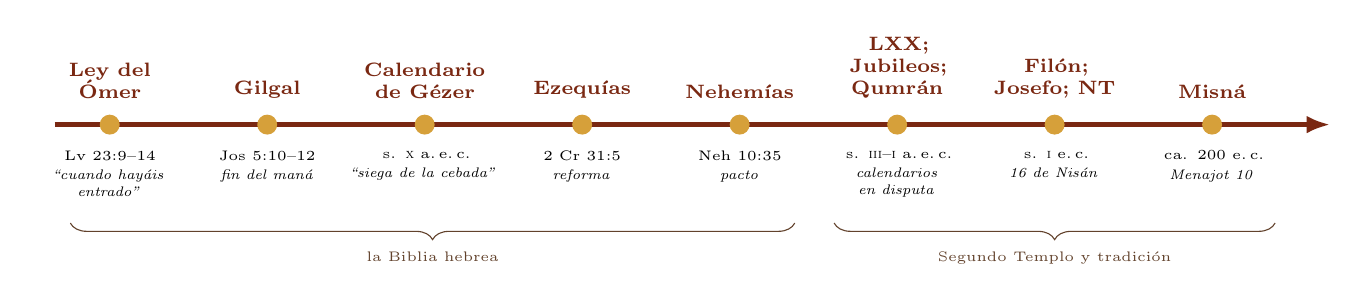
\begin{tikzpicture}[font=\scriptsize]
 \draw[line width=1.6pt,tierraroja,-{Latex[length=3mm]}] (0,0) -- (16.2,0);
 \foreach \x/\a/\b/\c in {0.7/{Ley del Ómer}/{Lv 23:9--14}/{``cuando hayáis entrado''}, 2.7/{Gilgal}/{Jos 5:10--12}/{fin del maná}, 4.7/{Calendario de Gézer}/{s. \textsc{x} a.\,e.\,c.}/{``siega de la cebada''}, 6.7/{Ezequías}/{2 Cr 31:5}/{reforma}, 8.7/{Nehemías}/{Neh 10:35}/{pacto}, 10.7/{LXX; Jubileos; Qumrán}/{s. \textsc{iii}--\textsc{i} a.\,e.\,c.}/{calendarios en disputa}, 12.7/{Filón; Josefo; NT}/{s. \textsc{i} e.\,c.}/{16 de Nisán}, 14.7/{Misná}/{ca. 200 e.\,c.}/{Menajot 10}}{
   \fill[mostaza] (\x,0) circle (3.6pt);
   \node[above=6pt,font=\scriptsize\bfseries,text=tierraroja,text width=1.85cm,align=center] at (\x,0) {\a};
   \node[below=6pt,text width=1.85cm,align=center,font=\tiny] at (\x,0) {\b\\[1pt]\textit{\c}};}
 \draw[decorate,decoration={brace,amplitude=6pt,mirror},sepia] (0.2,-1.25) -- (9.4,-1.25) node[midway,below=7pt,font=\tiny,text=sepia] {la Biblia hebrea};
 \draw[decorate,decoration={brace,amplitude=6pt,mirror},sepia] (9.9,-1.25) -- (15.5,-1.25) node[midway,below=7pt,font=\tiny,text=sepia] {Segundo Templo y tradición};
\end{tikzpicture}\par
{\footnotesize\color{sepia}\textit{Figura 2.} El Ómer y las primicias en la historia. \textit{Nota.} Elaboración propia. Las fechas de la ley y de Josué dependen de la cronología del éxodo (véase la precisión del §7).}
\end{center}

%===================================================================
\section{Lectura filológica}

El castellano ``primicias'' cubre un campo que el hebreo divide con más precisión. Seis palabras se cruzan en Levítico 23 y sus paralelos: \emph{ómer}, \emph{reshit}, \emph{bikurim}, \emph{terumá}, \emph{tenufá} y la fórmula \emph{lirtsonjem}. A ellas se suman sus equivalentes griegos, que son el puente hacia Pablo (léxicos: Brown et al., 1906; Koehler y Baumgartner, 2001; Bauer et al., 2000).

\subsection{\emph{Ómer}: medida y gavilla}

\begin{filologia}[\heb{עֹמֶר} (\emph{ómer})]
Sustantivo masculino con dos usos. (1) \emph{Medida} de áridos: ``un gomer por cabeza'' de maná (Éx 16:16), y la equivalencia explícita: \heb{וְהָעֹמֶר עֲשִׂרִית הָאֵיפָה הוּא}, ``y un gomer es la décima parte de un efa'' (Éx 16:36). Su volumen depende del valor que se asigne al efa (entre unos 22 y 36 litros según los autores), de modo que el ómer va de unos 2,2 a 3,6 litros; en mi presentación anterior sobre los Ázimos, siguiendo glosas judías, di ≈\,3.500\,cm³ de cebada. La RVR1960 transcribe ``gomer'' en Éxodo 16. (2) \emph{Gavilla} atada de espigas: Rut espiga ``entre las gavillas'' (\heb{בָעֳמָרִים}, Rut 2:7, 15); la ley del rebusco ordena dejar la gavilla olvidada en el campo (\heb{וְשָׁכַחְתָּ עֹמֶר בַּשָּׂדֶה}, Dt 24:19); Job habla de los pobres que llevan las gavillas con hambre (Job 24:10). En Lv 23:10--15 el sentido es ``gavilla'' (RVR1960), aunque la tradición rabínica, por el procedimiento de Lv 2:14, ofrecía en el altar una décima de efa de harina obtenida de ella.
\par\smallskip\emph{Conteo (morfología WLC, Strong H6016):} 14 apariciones: seis en Éx 16 (vv. 16, 18, 22, 32, 33, 36), cuatro en Lv 23 (vv. 10, 11, 12, 15), Dt 24:19, Rut 2:7, 15 y Job 24:10.
\end{filologia}

Para el lector bíblico, la coincidencia de los dos sentidos tiene algo que decir. El maná se medía por \emph{ómer} en el desierto; en la tierra, el primer \emph{ómer} de la siega se entregaba a Dios, y la medida del pan dado se vuelve la gavilla del pan cosechado. El texto no explicita ese juego, pero Josué 5:12 lo sugiere al hacer coincidir el fin del maná con el primer fruto de la tierra.

\subsection{\emph{Reshit}: lo primero y lo mejor}

\begin{filologia}[\heb{רֵאשִׁית} (\emph{reshit})]
De \heb{רֹאשׁ} (\emph{rosh}, ``cabeza''). Designa lo que va a la cabeza en el tiempo (``principio'') o en la calidad (``lo mejor, lo selecto''). Sentido temporal: \heb{בְּרֵאשִׁית} (Gn 1:1); ``el principio de la sabiduría es el temor de \SENOR'' (Pr 1:7; Sal 111:10). Sentido de calidad: los poderosos de Samaria ``se ungen con los ungüentos más preciosos'' (\heb{וְרֵאשִׁית שְׁמָנִים}, Am 6:6); los notables de Samaria, ``principales entre las naciones'' (\heb{רֵאשִׁית הַגּוֹיִם}, Am 6:1). Sentido cultual: \emph{reshit qetsirjem} (Lv 23:10), \emph{reshit arisotejem}, ``lo primero que amaséis'' (Nm 15:20), \emph{reshit tevuatejá}, ``las primicias de todos tus frutos'' (Pr 3:9). En Nm 18:12 \emph{reshit} es ``todo lo más escogido'' del aceite, el vino y el grano.
\par\smallskip LXX: casi siempre \grc{ἀπαρχή} en el sentido cultual; \grc{ἀρχή} en el temporal.
\end{filologia}

\subsection{\emph{Bikurim}: los primeros maduros}

\begin{filologia}[\heb{בִּכּוּרִים} (\emph{bikurim})]
De la raíz \heb{בכר}, ``ser primero, madurar temprano'', la misma de \heb{בְּכוֹר} (\emph{bejor}, ``primogénito'') y de \heb{בִּכּוּרָה} (\emph{bikurá}, ``breva, higo temprano'': ``como la fruta temprana de la higuera'', Os 9:10; Is 28:4). \emph{Bikurim} son los frutos que maduran antes que los demás (17 apariciones del plural en el Códice de Leningrado, más \emph{bikurá} en Is 28:4; \emph{reshit} aparece 51 veces). La fórmula de Éx 23:19 y 34:26 une las dos palabras: \heb{רֵאשִׁית בִּכּוּרֵי אַדְמָתְךָ}, ``las primicias de los primeros frutos de tu tierra''. Nm 18:12--13 las pone una tras otra: \emph{reshitam} (``las primicias de ello'') y \emph{bikuré kol asher beartsam} (``las primicias de todas las cosas de la tierra de ellos''). Shavuot es \heb{יוֹם הַבִּכּוּרִים} (\emph{yom habikurim}, Nm 28:26), ``el día de las primicias''.
\par\smallskip LXX: \grc{πρωτογενήματα} (Éx 23:19: \grc{τὰς ἀπαρχὰς τῶν πρωτογενημάτων τῆς γῆς σου}).
\end{filologia}

Las dos palabras se distinguen sin oponerse. \emph{Reshit} mira a la posición (lo que va primero y lo mejor de lo que hay); \emph{bikurim}, a la maduración (lo que madura antes). Que \emph{bikurim} comparta raíz con \emph{bejor} une el campo y la familia, pues el primogénito es el ``primer maduro'' de la casa; cuando Dios dice ``Israel es mi hijo, mi primogénito'' (\heb{בְּנִי בְכֹרִי יִשְׂרָאֵל}, Éx 4:22) usa la misma raíz con que la ley nombra los primeros frutos.

\subsection{\emph{Terumá} y \emph{tenufá}: lo alzado y lo mecido}

\begin{filologia}[\heb{תְּרוּמָה} (\emph{terumá})]
De \heb{רוּם}, ``ser alto, alzar''. Es lo ``alzado'', es decir, lo separado de un conjunto y apartado para Dios o para el santuario. La RVR1960 la traduce ``ofrenda'' (Éx 25:2, para el tabernáculo), ``ofrenda elevada'' (Nm 18:8) o ``primicias'' según el contexto. La torta de la primera masa es \emph{terumá} (Nm 15:20); el diezmo del diezmo de los levitas también (Nm 18:26). En la Misná, \emph{terumá} designa la porción de la cosecha que corresponde al sacerdote (tratado \emph{Terumot}).
\end{filologia}

\begin{filologia}[\heb{תְּנוּפָה} (\emph{tenufá}) y \heb{הֵנִיף} (\emph{heníf})]
De \heb{נוף}, en hifil ``mover, agitar, blandir''. Se blande una herramienta sobre la piedra (Éx 20:25), la hoz sobre la mies (Dt 23:25 [23:26]), la mano sobre el río (Is 11:15). En el culto, \emph{tenufá} es la ofrenda que el sacerdote ``mece delante del \SENOR'': el pecho del sacrificio de paz (Lv 7:30), la gavilla del Ómer (Lv 23:11, 15), los dos panes (Lv 23:17, 20). Sentido discutido: la tradición rabínica describe un movimiento hacia adelante y hacia atrás, arriba y abajo (Misná Menajot 5:6; tradición). Milgrom (1991) sostiene que el gesto es una \emph{elevación} que transfiere la ofrenda al dominio divino, y propone traducir ``ofrenda de elevación''. Su argumento más fuerte es Nm 8:11--21, donde Aarón ``ofrece'' a los levitas como \emph{tenufá}: difícilmente un balanceo físico; más bien una dedicación. La RVR1960 mantiene ``mecer''.
\end{filologia}

\subsection{\emph{Lirtsonjem}: ``para que seáis aceptos''}

\begin{filologia}[\heb{לִרְצֹנְכֶם} (\emph{lirtsonjem})]
De \heb{רָצוֹן} (\emph{ratsón}), ``agrado, aceptación, favor''. La fórmula técnica dice que una ofrenda es aceptada \emph{a favor} del oferente: ``de su voluntad lo ofrecerá'' (Lv 1:3, \emph{lirtsonó}, ``para su aceptación''); ``para que sea aceptado'' (Lv 22:20--21). En Lv 23:11 el sujeto aceptado es el pueblo; la gavilla es la condición de que Israel sea recibido con su cosecha. La LXX traduce \grc{δεκτὸν ὑμῖν}, ``aceptable para vosotros''. El mismo campo reaparece en ``el año de la buena voluntad del \SENOR'' (\heb{שְׁנַת־רָצוֹן}, Is 61:2), que Jesús lee en Nazaret como \grc{ἐνιαυτὸν κυρίου δεκτόν} (Lc 4:19), y en ``en tiempo aceptable te he oído'' (Is 49:8; 2~Co 6:2, \grc{καιρῷ δεκτῷ}).
\end{filologia}

\subsection{La Septuaginta: \emph{drágma} y \emph{aparjé}}

\begin{filologia}[\grc{δράγμα} y \grc{ἀπαρχή}]
La LXX traduce Lv 23:10 con dos palabras: \grc{δράγμα}, ``puñado, gavilla'' (lo que cabe en la mano del segador, de \grc{δράσσομαι}, ``agarrar''), y \grc{ἀπαρχή}, ``primicia''. \grc{Ἀπαρχή} viene de \grc{ἀπάρχομαι}, ``ofrecer las primicias'', ``empezar un sacrificio''; en el griego clásico designa la porción inicial que se aparta para los dioses. En la LXX traduce sobre todo \emph{reshit} y \emph{terumá}. En Lv 23:11 la LXX dice que el sacerdote ``elevará'' (\grc{ἀνοίσει}) la gavilla, un verbo que coincide con la lectura de Milgrom.
\end{filologia}

\begin{filologia}[\grc{ἀπαρχή} y \grc{πρωτότοκος} en el Nuevo Testamento]
\grc{Ἀπαρχή} aparece nueve veces en el NT según el SBLGNT, que coincide aquí con NA28 (ocho en Westcott-Hort, que lee \grc{ἀπ᾽ ἀρχῆς} en 2~Ts 2:13): Cristo resucitado (1~Co 15:20, 23); el Espíritu como anticipo (\grc{τὴν ἀπαρχὴν τοῦ πνεύματος}, Ro 8:23); las primicias de la masa (Ro 11:16, eco de Nm 15:20); los primeros convertidos de una región (Ro 16:5; 1~Co 16:15); la iglesia como ``primicias de sus criaturas'' (\grc{ἀπαρχήν τινα τῶν αὐτοῦ κτισμάτων}, Stg 1:18); los 144\,000, ``primicias para Dios y para el Cordero'' (Ap 14:4); y, según NA28, 2~Ts 2:13 (variante: §5.5). Junto a ella, \grc{πρωτότοκος} (``primogénito'', ocho veces en el SBLGNT) traduce \emph{bejor}: Cristo es ``el primogénito de entre los muertos'' (Col 1:18; Ap 1:5) y ``el primogénito entre muchos hermanos'' (Ro 8:29); la ``congregación de los primogénitos que están inscritos en los cielos'' (\grc{ἐκκλησίᾳ πρωτοτόκων}, He 12:23) es el texto que el documento de referencia usa para su primer período.
\end{filologia}

\subsection{El campo semántico}
El esquema siguiente reúne las palabras: en el centro, la idea común; alrededor, cada término con su matiz y un texto representativo.

\begin{center}
\begin{tikzpicture}[font=\scriptsize,
  t/.style={draw=tierraroja!70,line width=0.6pt,fill=papiro,rounded corners=2pt,text width=3.25cm,align=center,inner sep=4pt}]
 \node[draw=tierraroja,line width=1pt,fill=mostaza!25,rounded corners=4pt,text width=3.4cm,align=center,inner sep=6pt] (c) at (0,0)
   {\small\bfseries\color{tierraroja} Lo primero\\ pertenece a Dios\\[2pt]\normalfont\tiny\color{sepia}y consagra el resto (Ro 11:16)};
 \node[t] (r) at (-5.1,1.9) {\heb{רֵאשִׁית} \textbf{reshit}\\ lo primero y lo mejor\\ \textit{Lv 23:10; Pr 3:9}};
 \node[t] (b) at (0,2.65) {\heb{בִּכּוּרִים} \textbf{bikurim}\\ los primeros maduros\\ \textit{Éx 23:19; Nm 28:26}};
 \node[t] (k) at (5.1,1.9) {\heb{בְּכוֹר} \textbf{bejor}\\ el primogénito\\ \textit{Éx 4:22; 13:2}};
 \node[t] (o) at (-5.1,-1.9) {\heb{עֹמֶר} \textbf{ómer}\\ gavilla; décima de efa\\ \textit{Lv 23:10; Éx 16:36}};
 \node[t] (n) at (0,-2.65) {\heb{תְּנוּפָה} \textbf{tenufá}\\ lo mecido o elevado\\ \textit{Lv 23:11, 15; Nm 8:11}};
 \node[t] (m) at (5.1,-1.9) {\heb{תְּרוּמָה} \textbf{terumá}\\ lo alzado y separado\\ \textit{Nm 15:20; 18:8}};
 \foreach \n in {r,b,k,o,n,m} \draw[sepia!80,line width=0.5pt] (c) -- (\n);
 \draw[mostaza!90!tierraroja,line width=0.8pt,dashed,{Latex[length=2mm]}-{Latex[length=2mm]}] (b.east) to[bend left=12] node[above,font=\tiny,text=sepia]{raíz \heb{בכר}} (k.north);
\end{tikzpicture}\par
{\footnotesize\color{sepia}\textit{Figura 3.} El campo semántico de las primicias. \textit{Nota.} Elaboración propia; la línea discontinua une las palabras de la misma raíz.}
\end{center}

El puente léxico es directo. El hebreo \emph{reshit} pasa a la LXX como \grc{ἀπαρχή}, y Pablo, que lee la Biblia griega, toma esa palabra para nombrar a Cristo resucitado; cuando escribe \grc{ἀπαρχὴ τῶν κεκοιμημένων} no está inventando una metáfora agrícola, sino usando el término técnico de la gavilla de Levítico.

\begin{center}
\begin{tikzpicture}[font=\scriptsize,
  b/.style={draw=tierraroja,line width=0.8pt,fill=papiro,rounded corners=3pt,text width=3.25cm,align=center,inner sep=5pt,minimum height=2.3cm}]
 \node[b] (h) at (0,0) {\textbf{\color{tierraroja}Hebreo (Lv 23:10)}\\[3pt]\heb{עֹמֶר רֵאשִׁית קְצִירְכֶם}\\[2pt]\emph{ómer reshit qetsirjem}\\ ``gavilla, primicia de vuestra siega''};
 \node[b] (g) at (4.15,0) {\textbf{\color{tierraroja}LXX (Lv 23:10)}\\[3pt]\grc{δράγμα ἀπαρχὴν τοῦ θερισμοῦ ὑμῶν}\\[2pt]``gavilla, primicia de vuestra siega''};
 \node[b] (p) at (8.3,0) {\textbf{\color{tierraroja}Pablo (1 Co 15:20)}\\[3pt]\grc{ἀπαρχὴ τῶν κεκοιμημένων}\\[2pt]``primicia de los que han dormido''};
 \node[b] (e) at (12.45,0) {\textbf{\color{tierraroja}RVR1960}\\[3pt]``primicias de los que durmieron es hecho''\\[2pt]cf. Mt 27:52 \grc{τῶν κεκοιμημένων ἁγίων}};
 \foreach \a/\b in {h/g,g/p,p/e} \draw[-{Latex[length=2.5mm]},line width=1.2pt,mostaza] (\a) -- (\b);
 \node[font=\scriptsize\itshape,text=sepia,text width=15cm,align=center] at (6.2,-1.75) {La gavilla que abría la siega se convierte en el nombre de Cristo resucitado, que abre la resurrección de ``los que durmieron''.};
\end{tikzpicture}\par
{\footnotesize\color{sepia}\textit{Figura 4.} De la gavilla de Levítico a la primicia de Pablo. \textit{Nota.} Elaboración propia: BHS, LXX (Rahlfs-Hanhart) y NA28.}
\end{center}

%===================================================================
\section{Lectura textual: el día siguiente del sábado}\label{sec:textual}

\subsection{El problema}
Lv 23:11 no da una fecha. Los demás tiempos de la primavera tienen número: ``a los catorce del mes'' la Pascua, ``a los quince días de este mes'' los Ázimos (Lv 23:5--6). El Ómer, en cambio, se ofrece \heb{מִמָּחֳרַת הַשַּׁבָּת} (\emph{mimojorat hashabat}), ``el día siguiente del sábado''. ¿Qué sábado? La pregunta dividió a los judíos del Segundo Templo y sigue dividiendo a las comunidades que guardan las fiestas, y es textual en sentido estricto, porque todo depende de qué significa \emph{shabat} en este capítulo.

\subsection{Las tres lecturas}

\paragraph{1. Fariseos y rabinos: el día siguiente del primer día festivo (16 de Nisán).} ``Sábado'' designa aquí el primer día de los Ázimos, el 15 de Abib, que es día de reposo aunque no caiga en el séptimo día de la semana. El Ómer se ofrece siempre el 16 de Nisán, cualquiera sea el día de la semana, y Shavuot cae el 6 de Siván. El apoyo de esta lectura es antiguo y amplio: la LXX traduce Lv 23:11 \grc{τῇ ἐπαύριον τῆς πρώτης}, ``el día siguiente del primero'' [día]; el Targum Onqelos, \emph{mibatar yoma tava}, ``después del día festivo'' (verificar); Filón (\emph{Spec.} 2.162) y Josefo (\emph{Ant.} 3.250) dan el 16. La Misná y el Talmud la defienden contra los boetusianos (Menajot 10:3; Talmud de Babilonia, Menajot 65a--66a).

\paragraph{2. Saduceos y boetusianos: el domingo dentro de la semana de los Ázimos.} ``Sábado'' es el sábado semanal que cae durante los siete días de los Ázimos; el Ómer se ofrece el domingo siguiente, que puede caer entre el 16 y el 22 de Nisán. Pentecostés cae siempre en domingo, con fecha variable. La Misná atribuye esta posición a los boetusianos; la sostuvieron después los caraítas (desde el siglo \textsc{viii}) y los samaritanos. La practican también varias iglesias de tradición sabatista, entre ellas la Iglesia de Dios Unida, cuyo calendario fija Pentecostés siempre en domingo (Iglesia de Dios Unida, 2011).

\paragraph{3. Qumrán y Jubileos: el domingo después de la semana de los Ázimos (26 del mes primero).} El calendario solar de 364 días, atestiguado en Jubileos y en los manuscritos del mar Muerto, hace caer cada fecha siempre en el mismo día de la semana. El año empieza en miércoles; el 14 del mes primero es martes, el 15 miércoles, y el sábado posterior a la semana festiva es el 25. El \emph{Rollo del Templo} (11Q19 18--19) fija la ofrenda de la gavilla el domingo 26, y Shavuot cae el 15 del tercer mes, la fecha que Jubileos asigna a la fiesta del pacto (Jub 6:17--21; 15:1; Yadin, 1983; VanderKam, 1998).

\begin{center}\begin{minipage}{\linewidth}\centering\footnotesize\renewcommand{\arraystretch}{1.15}
\begin{tabular}{@{}L{3.2cm}L{3.3cm}L{2.2cm}L{2.5cm}L{3.2cm}@{}}
\toprule
\textbf{Grupo} & \textbf{``Sábado'' de Lv 23:11} & \textbf{Ómer} & \textbf{Shavuot} & \textbf{Testimonios} \\ \midrule
Fariseos, rabinos & primer día de Ázimos (15 Nisán) & 16 Nisán, día variable de la semana & 6 Siván, día variable & LXX; Onqelos; Filón; Josefo; Misná \\
Saduceos, boetusianos, caraítas, samaritanos & sábado semanal dentro de los Ázimos & domingo entre 16 y 22 & siempre domingo, fecha variable & Misná Menajot 10:3 (como adversarios); Anán ben David \\
Qumrán, Jubileos & sábado semanal después de los Ázimos & domingo 26 del mes I & domingo 15 del mes III & 11Q19 18--19; Jub 6; 4Q320--321 \\
\bottomrule
\end{tabular}\par
{\footnotesize\color{sepia}\textit{Tabla 3.} Las tres lecturas de \emph{mimojorat hashabat}. \textit{Nota.} Elaboración propia a partir de Milgrom (2001), VanderKam (1998) y Danby (1933).}
\end{minipage}\end{center}

El diagrama sitúa las tres fechas sobre el mes de Abib en un año en que el 15 cae en miércoles, como ocurre siempre en el calendario de Qumrán:

\begin{center}
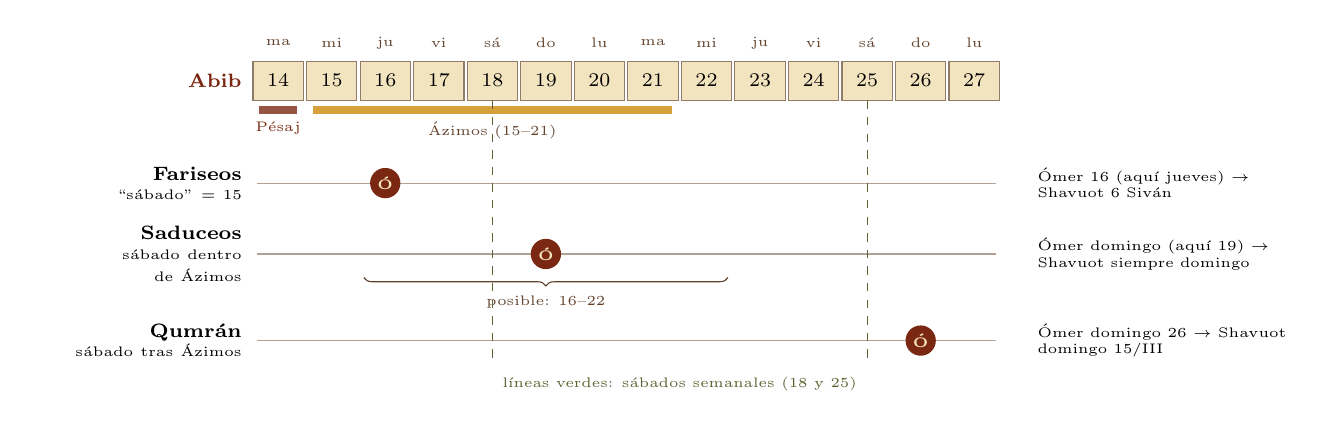
\begin{tikzpicture}[x=0.68cm,y=1cm,font=\scriptsize]
 % cabecera de días
 \foreach \d [count=\i from 0] in {14,15,16,17,18,19,20,21,22,23,24,25,26,27}{
   \node[draw=sepia!70,fill=papiro,minimum width=0.64cm,minimum height=0.5cm,inner sep=0pt] at (\i,0) {\d};}
 \foreach \w [count=\i from 0] in {ma,mi,ju,vi,sá,do,lu,ma,mi,ju,vi,sá,do,lu}{
   \node[font=\tiny,text=sepia] at (\i,0.48) {\w};}
 \node[anchor=east,font=\scriptsize\bfseries,text=tierraroja] at (-0.5,0) {Abib};
 % banda de Pésaj y Ázimos
 \fill[tierraroja!80] (-0.35,-0.42) rectangle (0.35,-0.32);
 \node[font=\tiny,text=tierraroja,below] at (0,-0.40) {Pésaj};
 \fill[mostaza] (0.65,-0.42) rectangle (7.35,-0.32);
 \node[font=\tiny,text=sepia,below] at (4,-0.40) {Ázimos (15--21)};
 % fila 1 fariseos
 \node[anchor=east,text width=2.6cm,align=right] at (-0.5,-1.3) {\textbf{Fariseos}\\[-1pt]\tiny ``sábado'' = 15};
 \draw[sepia!50] (-0.4,-1.3) -- (13.4,-1.3);
 \node[circle,fill=tierraroja,text=papiro,inner sep=1.3pt,font=\tiny\bfseries] at (2,-1.3) {Ó};
 \node[anchor=west,font=\tiny,text width=3.4cm] at (14,-1.3) {Ómer 16 (aquí jueves) $\rightarrow$ Shavuot 6 Siván};
 % fila 2 saduceos
 \node[anchor=east,text width=2.6cm,align=right] at (-0.5,-2.2) {\textbf{Saduceos}\\[-1pt]\tiny sábado dentro de Ázimos};
 \draw[sepia!50] (-0.4,-2.2) -- (13.4,-2.2);
 \draw[decorate,decoration={brace,amplitude=3pt,mirror},sepia] (1.6,-2.5) -- (8.4,-2.5) node[midway,below=3pt,font=\tiny]{posible: 16--22};
 \node[circle,fill=tierraroja,text=papiro,inner sep=1.3pt,font=\tiny\bfseries] at (5,-2.2) {Ó};
 \node[anchor=west,font=\tiny,text width=3.4cm] at (14,-2.2) {Ómer domingo (aquí 19) $\rightarrow$ Shavuot siempre domingo};
 % fila 3 qumran
 \node[anchor=east,text width=2.6cm,align=right] at (-0.5,-3.3) {\textbf{Qumrán}\\[-1pt]\tiny sábado tras Ázimos};
 \draw[sepia!50] (-0.4,-3.3) -- (13.4,-3.3);
 \node[circle,fill=tierraroja,text=papiro,inner sep=1.3pt,font=\tiny\bfseries] at (12,-3.3) {Ó};
 \node[anchor=west,font=\tiny,text width=3.4cm] at (14,-3.3) {Ómer domingo 26 $\rightarrow$ Shavuot domingo 15/III};
 % sábados semanales
 \foreach \s in {4,11}{\draw[oliva,dashed] (\s,-0.25) -- (\s,-3.6);}
 \node[font=\tiny,text=oliva] at (7.5,-3.85) {líneas verdes: sábados semanales (18 y 25)};
\end{tikzpicture}\par
{\footnotesize\color{sepia}\textit{Figura 5.} El mes de Abib y las tres fechas del Ómer (Ó). \textit{Nota.} Elaboración propia. Año ilustrativo con el 15 en miércoles; en el calendario fariseo el 16 cae en cualquier día de la semana, y la lectura saducea da domingo entre el 16 y el 22.}
\end{center}

\subsection{Los argumentos del texto}
Cada lectura tiene argumentos internos, y ninguna se impone sin discusión. A favor del sábado semanal: en el resto de Levítico 23, \emph{shabat} sin calificativo es el séptimo día (v. 3); el v. 15 habla de ``siete \emph{shabatot} cumplidos'' y el v. 16 del ``séptimo \emph{shabat}'', lo que parece contar semanas de sábado a sábado; y el texto no dice ``el día siguiente de la fiesta'', que habría sido más claro si esa fuera la intención. A favor del primer día festivo: Levítico llama \emph{shabatón} a días festivos que no son el séptimo día (vv. 24, 39) y \emph{shabat shabatón} a Yom Kipur, ``que es el diez del mes'' (vv. 27, 32); \emph{shabat} puede significar ``semana'' (las ``siete \emph{shabatot}'' de Lv 25:8 son semanas de años, y Dt 16:9 dice \emph{shavuot}, ``semanas''); y la ley pide una fecha fija, como las demás, que solo se obtiene si el ``sábado'' es el 15. A favor de Qumrán: si ``el sábado'' es el semanal y debe caer \emph{después} de los Ázimos completos, la gavilla no interrumpe la fiesta, y el calendario de 364 días fija a la vez la fecha y el día de la semana.

Los comentarios modernos coinciden en que el texto, aislado, no zanja la cuestión (Wenham, 1979; Levine, 1989; Hartley, 1992; Milgrom, 2001). Lo que sí está claro es la consecuencia: como el v. 16 usa la misma fórmula para el final de la cuenta, la definición del ``sábado'' de Lv 23:11 decide también el día de Pentecostés.

\begin{nota}[Precisión textual: la Septuaginta en Lv 23:11 y 23:15]
La LXX no es uniforme. En Lv 23:11 traduce ``el día siguiente del \emph{primero}'' (\grc{τῇ ἐπαύριον τῆς πρώτης}), lo que interpreta el texto en la línea farisea. En Lv 23:15--16 vuelve a la traducción literal: \grc{ἀπὸ τῆς ἐπαύριον τῶν σαββάτων}, ``desde el día siguiente de los sábados''. La versión griega es así el testimonio más antiguo de la lectura del 16 de Nisán, y a la vez muestra que los traductores sintieron la necesidad de aclarar un texto ambiguo. La RVR1960 traduce el TM: ``el día siguiente del día de reposo''.
\end{nota}

\subsection{Gilgal y ``el otro día de la pascua''}
Jos 5:11 dice que Israel comió el grano nuevo \heb{מִמָּחֳרַת הַפֶּסַח} (\emph{mimojorat hapésaj}), ``al otro día de la pascua''. La misma expresión aparece en Nm 33:3, donde designa el 15 de Abib: ``a los quince días del mes primero; el segundo día de la pascua salieron los hijos de Israel''. Si se lee Jos 5:11 con Nm 33:3, Israel habría comido grano tostado el 15, antes de cualquier Ómer; la tradición rabínica entiende ``pésaj'' en Josué como el día festivo del 15 y sitúa la comida el 16, después de la gavilla. La LXX no trae la frase ``al otro día de la pascua'' en Jos 5:11; dice que comieron ``panes ázimos y [grano] nuevo en este mismo día'' (\grc{ἄζυμα καὶ νέα ἐν ταύτῃ τῇ ἡμέρᾳ}). El pasaje no resuelve el debate, pero muestra que el narrador de Josué piensa la primera comida de la tierra en estrecha relación con la Pascua y con la ley de Lv 23:14.

\subsection{Variantes en el Nuevo Testamento}

\begin{nota}[Precisión textual: 2 Ts 2:13, ``desde el principio'' o ``como primicias'']
En 2~Ts 2:13 los manuscritos se dividen entre \grc{ἀπ᾽ ἀρχῆς} (``desde el principio'': Sinaítico, Beza, el texto mayoritario) y \grc{ἀπαρχήν} (``como primicias'': Vaticano, minúsculo 33, Vulgata). La diferencia en mayúsculas continuas es mínima: \grc{ΑΠΑΡΧΗΝ} frente a \grc{ΑΠΑΡΧΗΣ}. NA28 imprime \grc{ἀπαρχήν}: ``Dios os escogió como primicias para salvación''. La RVR1960 sigue la otra lectura: ``Dios os haya escogido desde el principio para salvación''. Si se acepta la lectura de NA28, Pablo llama primicias a los tesalonicenses como en Ro 16:5 llama primicia a Epeneto. Sobre la autoría de 2~Tesalonicenses, discutida por parte de la crítica, véase la nota del §8.
\end{nota}

\begin{nota}[Precisión textual: Ro 16:5 y Lc 6:1]
En Ro 16:5 Epeneto es ``el primer fruto (\grc{ἀπαρχή}) de Acaya para Cristo'' en la RVR1960, que sigue el texto mayoritario (\grc{Ἀχαΐας}); NA28 lee ``de Asia'' (\grc{Ἀσίας}), con los manuscritos más antiguos. En Lc 6:1, el episodio de los discípulos que arrancan espigas, buena parte de la tradición bizantina lee \grc{ἐν σαββάτῳ δευτεροπρώτῳ}, ``en un sábado segundo-primero'' (la Reina-Valera de 1909: ``en un sábado segundo del primero''); NA28 y la RVR1960 omiten el adjetivo, ausente en los manuscritos más antiguos. Desde Escalígero, algunos intérpretes propusieron que ``segundo-primero'' designaba el primer sábado después del segundo día de Pascua, es decir, el primero de la cuenta del ómer, lo que explicaría que hubiera espigas maduras y lícitas de comer. Es una hipótesis antigua sin consenso.
\end{nota}



%===================================================================
\section{Lectura literaria}

\subsection{Lv 23:9 abre una nueva unidad}
Levítico 23 está organizado por discursos divinos. Cada uno empieza con la misma fórmula, ``Y habló \SENOR{} a Moisés, diciendo'' (vv. 1, 9, 23, 26, 33):
\hebverso{וַיְדַבֵּר יְהוָה אֶל־מֹשֶׁה לֵּאמֹר}
\noindent La fórmula no aparece en el v. 15, de modo que el Ómer y Shavuot pertenecen al \emph{mismo} discurso (vv. 9--22): una sola ley con dos extremos, la gavilla de cebada y los dos panes de trigo, unidos por la cuenta. A la vez, una nueva introducción separa el Ómer de los Ázimos (vv. 4--8), aunque se celebre dentro de su semana. La estructura dice lo que el calendario oculta: la gavilla mira hacia adelante, a la siega que culmina en Pentecostés.

\begin{center}
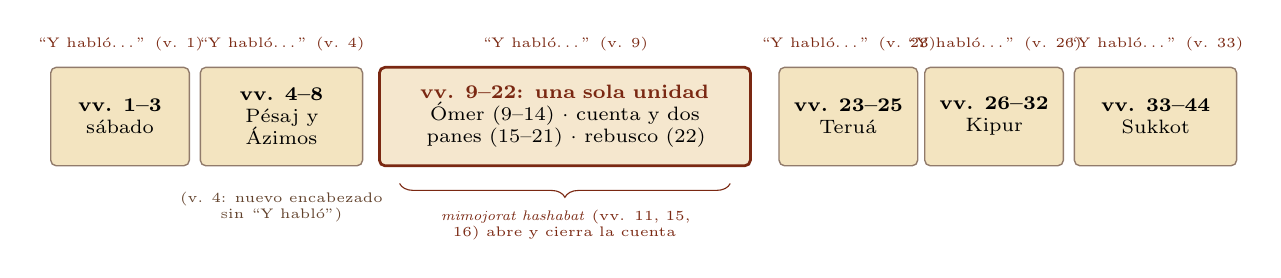
\begin{tikzpicture}[font=\scriptsize,
  u/.style={draw=sepia!70,line width=0.5pt,fill=papiro,rounded corners=2pt,minimum height=1.25cm,align=center,inner sep=3pt},
  h/.style={draw=tierraroja,line width=1pt,fill=mostaza!25,rounded corners=2pt,minimum height=1.25cm,align=center,inner sep=3pt}]
 \node[u,text width=1.55cm] (a) at (0,0) {\textbf{vv. 1--3}\\ sábado};
 \node[u,text width=1.85cm] (b) at (2.05,0) {\textbf{vv. 4--8}\\ Pésaj y Ázimos};
 \node[h,text width=4.5cm] (c) at (5.65,0) {\textbf{\color{tierraroja}vv. 9--22: una sola unidad}\\ Ómer (9--14) $\cdot$ cuenta y dos panes (15--21) $\cdot$ rebusco (22)};
 \node[u,text width=1.55cm] (d) at (9.25,0) {\textbf{vv. 23--25}\\ Teruá};
 \node[u,text width=1.55cm] (e) at (11.1,0) {\textbf{vv. 26--32}\\ Kipur};
 \node[u,text width=1.85cm] (f) at (13.15,0) {\textbf{vv. 33--44}\\ Sukkot};
 \foreach \n/\v in {a/1,b/4,c/9,d/23,e/26,f/33}{
   \node[font=\tiny,text=tierraroja] at ([yshift=8pt]\n.north) {``Y habló\ldots'' (v. \v)};}
 \node[font=\tiny,text=sepia,align=center] at (2.05,-1.15) {(v. 4: nuevo encabezado\\ sin ``Y habló'')};
 \draw[decorate,decoration={brace,amplitude=5pt,mirror},tierraroja] (3.55,-0.85) -- (7.75,-0.85) node[midway,below=6pt,font=\tiny,text=tierraroja,text width=4.6cm,align=center]{\emph{mimojorat hashabat} (vv. 11, 15, 16) abre y cierra la cuenta};
\end{tikzpicture}\par
{\footnotesize\color{sepia}\textit{Figura 6.} Los discursos de Levítico 23. \textit{Nota.} Elaboración propia sobre la BHS. La fórmula ``Y habló \SENOR{} a Moisés'' aparece en los vv. 1, 9, 23, 26 y 33.}
\end{center}

\subsection{Una ley para la tierra futura}
La cláusula ``cuando hayáis entrado en la tierra que yo os doy'' (\heb{כִּי־תָבֹאוּ אֶל־הָאָרֶץ}) aparece en Levítico solo en leyes que dependen de la tierra: la lepra de las casas (Lv 14:34), los frutos de los árboles nuevos, que no se comen los tres primeros años y se consagran el cuarto (Lv 19:23--25), y el año sabático de la tierra (Lv 25:2). Las tres comparten con el Ómer la misma idea: la tierra es de Dios y el israelita la recibe como arrendatario (``la tierra mía es; pues vosotros forasteros y extranjeros sois para conmigo'', Lv 25:23). La ley de Lv 19:23--25 es la más cercana, porque ``el cuarto año todo su fruto será consagrado en alabanzas a \SENOR'' (Lv 19:24) y solo entonces se come del árbol; el Ómer aplica esa misma lógica a cada año agrícola.

\subsection{La bisagra entre Pascua y Pentecostés}
Por la fecha, el Ómer pertenece a los Ázimos; por la estructura literaria y por la cuenta, a Shavuot. Las dos ofrendas mecidas de la primavera se corresponden y se contrastan:

\begin{center}
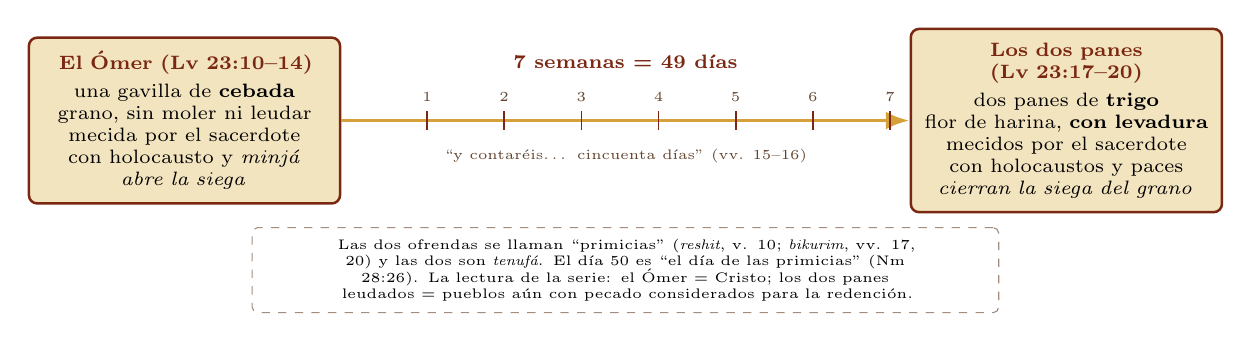
\begin{tikzpicture}[font=\scriptsize,
  g/.style={draw=tierraroja,line width=0.9pt,fill=papiro,rounded corners=3pt,text width=3.6cm,align=center,inner sep=5pt}]
 \node[g] (o) at (0,0) {\textbf{\color{tierraroja}El Ómer (Lv 23:10--14)}\\[2pt] una gavilla de \textbf{cebada}\\ grano, sin moler ni leudar\\ mecida por el sacerdote\\ con holocausto y \emph{minjá}\\ \textit{abre la siega}};
 \node[g] (p) at (11.2,0) {\textbf{\color{tierraroja}Los dos panes (Lv 23:17--20)}\\[2pt] dos panes de \textbf{trigo}\\ flor de harina, \textbf{con levadura}\\ mecidos por el sacerdote\\ con holocaustos y paces\\ \textit{cierran la siega del grano}};
 \draw[line width=1.4pt,mostaza,-{Latex[length=3mm]}] (o.east) -- (p.west);
 \foreach \i in {1,...,7}{
   \pgfmathsetmacro{\xx}{2.1+\i*0.98}
   \draw[tierraroja,line width=0.6pt] (\xx,-0.12) -- (\xx,0.12);
   \node[font=\tiny,text=sepia] at (\xx,0.3) {\i};}
 \node[font=\scriptsize\bfseries,text=tierraroja] at (5.6,0.75) {7 semanas = 49 días};
 \node[font=\tiny,text=sepia] at (5.6,-0.45) {``y contaréis\ldots{} cincuenta días'' (vv. 15--16)};
 \node[draw=sepia!60,dashed,rounded corners=2pt,text width=9.2cm,align=center,font=\tiny,inner sep=4pt] at (5.6,-1.9)
   {Las dos ofrendas se llaman ``primicias'' (\emph{reshit}, v. 10; \emph{bikurim}, vv. 17, 20) y las dos son \emph{tenufá}. El día 50 es ``el día de las primicias'' (Nm 28:26). La lectura de la serie: el Ómer = Cristo; los dos panes leudados = pueblos aún con pecado considerados para la redención.};
\end{tikzpicture}\par
{\footnotesize\color{sepia}\textit{Figura 7.} De la gavilla a los dos panes: la cuenta como puente entre fiestas. \textit{Nota.} Elaboración propia; la última línea resume el documento de referencia (lección 11).}
\end{center}

La gavilla se ofrece en su forma más simple y temprana; los panes, en la más elaborada y cotidiana, con levadura, que estaba excluida del altar (Lv 2:11). Por eso los panes de Shavuot no se quemaban, sino que se mecían y quedaban para los sacerdotes (Lv 23:20). El arco de cincuenta días lleva del grano que acaba de brotar al pan que se come en casa.

\subsection{Heptadas: de la cuenta del ómer al jubileo}
La cuenta del Ómer tiene un paralelo exacto en la ley del jubileo: los dos textos usan el mismo verbo, la misma construcción reflexiva (``contaréis \emph{para vosotros}'') y la misma unidad, siete \emph{shabatot}.

\hebverso{וּסְפַרְתֶּם לָכֶם \foreignlanguage{spanish}{[\ldots]} שֶׁבַע שַׁבָּתוֹת תְּמִימֹת \\ וְסָפַרְתָּ לְךָ שֶׁבַע שַׁבְּתֹת שָׁנִים}
\begin{cita}Y contaréis desde el día que sigue al día de reposo\ldots{} siete semanas cumplidas serán.\fuente{(Lv 23:15)}\\
Y contarás siete semanas de años, siete veces siete años, de modo que los días de las siete semanas de años vendrán a serte cuarenta y nueve años\ldots{} Y santificaréis el año cincuenta.\fuente{(Lv 25:8, 10)}\end{cita}

Lo que el Ómer hace con los días, el jubileo lo hace con los años: siete por siete, y luego el quincuagésimo, que es libertad (Lv 25:10, \emph{derór}) y regreso a la tierra. La serie, que integra el jubileo y la \emph{shemitá} en su lectura del calendario, encuentra aquí un apoyo literario sólido, pues la cuenta que empieza con la primera gavilla es una miniatura anual del gran ciclo de la tierra. La conexión es léxica y estructural; su sentido tipológico (el jubileo como figura de la redención final) es una lectura posterior, que el estudio del jubileo marcará como tal.

\subsection{El patrón ``lo primero para Dios''}
La gavilla no es una ley aislada. Desde el primer culto narrado en la Biblia, Dios reclama lo primero, y lo primero consagra lo demás. Abel ``trajo también de los primogénitos de sus ovejas, de lo más gordo de ellas. Y miró \SENOR{} con agrado a Abel y a su ofrenda'' (Gn 4:4); el texto contrasta su ofrenda, descrita con dos marcas de calidad (\emph{bejorot}, \emph{jelev}), con la de Caín, que trajo ``del fruto de la tierra'' sin calificativos (Gn 4:3). La misma lógica vuelve en el primogénito (Éx 13:2), las primicias del campo (Éx 23:19), la masa (Nm 15:20), los bienes (Pr 3:9) y, al final, en las personas: Israel, Cristo y la iglesia.

\begin{center}
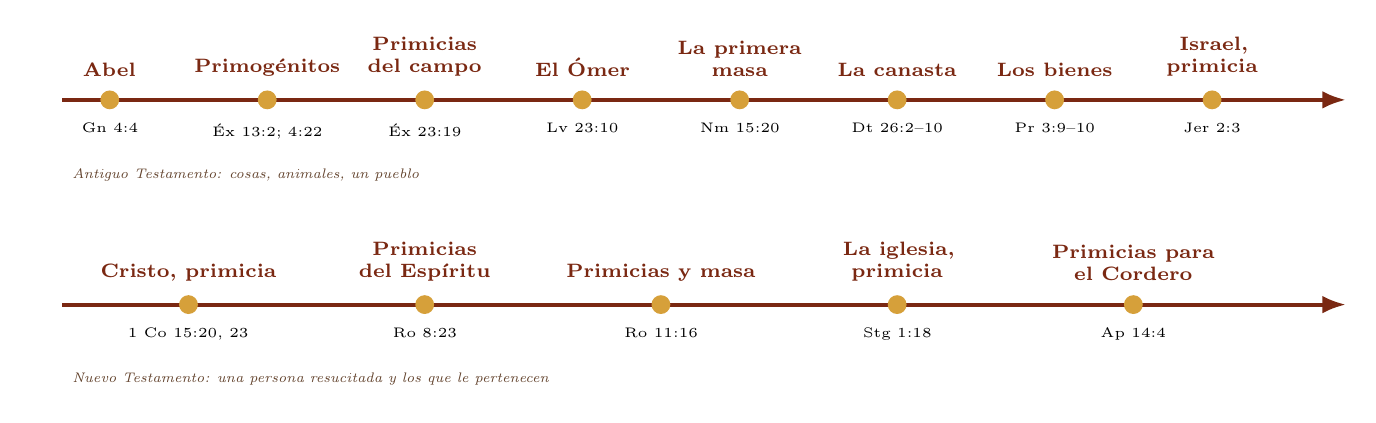
\begin{tikzpicture}[font=\scriptsize]
 \draw[line width=1.4pt,tierraroja,-{Latex[length=3mm]}] (0,0) -- (16.3,0);
 \foreach \x/\a/\b in {0.6/{Abel}/{Gn 4:4}, 2.6/{Primogénitos}/{Éx 13:2; 4:22}, 4.6/{Primicias del campo}/{Éx 23:19}, 6.6/{El Ómer}/{Lv 23:10}, 8.6/{La primera masa}/{Nm 15:20}, 10.6/{La canasta}/{Dt 26:2--10}, 12.6/{Los bienes}/{Pr 3:9--10}, 14.6/{Israel, primicia}/{Jer 2:3}}{
   \fill[mostaza] (\x,0) circle (3.4pt);
   \node[above=5pt,font=\scriptsize\bfseries,text=tierraroja,text width=1.85cm,align=center] at (\x,0) {\a};
   \node[below=5pt,font=\tiny,text width=1.85cm,align=center] at (\x,0) {\b};}
 \begin{scope}[yshift=-2.6cm]
 \draw[line width=1.4pt,tierraroja,-{Latex[length=3mm]}] (0,0) -- (16.3,0);
 \foreach \x/\a/\b in {1.6/{Cristo, primicia}/{1 Co 15:20, 23}, 4.6/{Primicias del Espíritu}/{Ro 8:23}, 7.6/{Primicias y masa}/{Ro 11:16}, 10.6/{La iglesia, primicia}/{Stg 1:18}, 13.6/{Primicias para el Cordero}/{Ap 14:4}}{
   \fill[mostaza] (\x,0) circle (3.4pt);
   \node[above=5pt,font=\scriptsize\bfseries,text=tierraroja,text width=2.4cm,align=center] at (\x,0) {\a};
   \node[below=5pt,font=\tiny,text width=2.2cm,align=center] at (\x,0) {\b};}
 \end{scope}
 \node[anchor=west,font=\tiny\itshape,text=sepia] at (0,-0.95) {Antiguo Testamento: cosas, animales, un pueblo};
 \node[anchor=west,font=\tiny\itshape,text=sepia] at (0,-3.55) {Nuevo Testamento: una persona resucitada y los que le pertenecen};
\end{tikzpicture}\par
{\footnotesize\color{sepia}\textit{Figura 8.} El patrón ``lo primero para Dios'' en la Escritura. \textit{Nota.} Elaboración propia.}
\end{center}

Pablo formula el principio en una línea: ``Si las primicias son santas, también lo es la masa restante'' (\grc{εἰ δὲ ἡ ἀπαρχὴ ἁγία, καὶ τὸ φύραμα}, Ro 11:16). La imagen viene de Nm 15:20--21, la torta de la primera masa, que la LXX llama \grc{ἀπαρχὴν φυράματος}. La primicia no es una muestra cualquiera, sino la parte que, entregada a Dios, hace santo al todo. Así hay que leer también la gavilla del Ómer: no paga la cosecha, la consagra, y ``para que seáis aceptos'' (Lv 23:11) dice a quién consagra.

%===================================================================
\section{Memorial, figura y esperanza: la lectura de la serie}\label{sec:serie}

\subsection{El marco: Reglamento de Culto y tres períodos}
El documento de referencia de la serie lee Levítico 23 como el ``Reglamento del Culto'' instituido por Dios: las solemnidades del \SENOR, proclamadas ``convocaciones santas'', ``en sus tiempos'', ``estatuto perpetuo''. Lo distingue de la ``Ley de los sacrificios'' o ``mandamientos en orden a ritos'' (Nm 28--29; Lv 1--7). Cada fiesta, sostiene, es memorial de un hito histórico de Israel en su marcha hacia la tierra y figura del plan de salvación. El Ómer ocupa un lugar especial en ese esquema, y el documento le dedica una ``mención aparte'':

\begin{cita}Mención aparte merece la ceremonia de la presentación del Omer, que sin ser un día de guardar la gavilla del Omer fue una ``ofrenda de primicias'' con un profundo contenido espiritual\ldots{} [que] en el período del Primer pacto representó al pueblo de Israel, cuando luego de cruzar el Mar Rojo se constituye como la primicia de las naciones del mundo rescatadas para Dios (Éxodo 19:5 y 6). Del mismo modo en la era del Nuevo Pacto, representa el sacrificio de nuestro Señor, que constituye al Hijo de Dios la primicia de los resucitados para vida eterna.\fuente{(Documento de referencia, lección 8)}\end{cita}

La tesis tiene tres partes, que las subsecciones siguientes toman por separado: un \emph{memorial} (Israel primicia de las naciones), una \emph{figura} (Cristo primicia de los resucitados, recibido a la diestra del Padre) y una consecuencia sobre la \emph{vigencia} del rito.

\subsection{Memorial: Israel, primicia de las naciones}
La lección 7 reconstruye la secuencia del éxodo: el pueblo fue librado de la muerte (Pascua) y salió de la tierra del cautiverio (Ázimos), pero ``aún no estaban libres del faraón''. Siguiendo Nm 33:1--7 y Éx 14, el documento propone este itinerario: el 15 de Abib los israelitas salen de Gosén y Ramesés y acampan en Sucot; el 16 marchan a Etam; el 17 llegan a Migdol, junto al mar, donde los alcanza el faraón, ``y en este mismo día'' cruzan el mar. De ahí concluye:

\begin{cita}De modo que, no es erróneo afirmar que el siguiente día, el día 18 de Abib, Israel puede presentarse, por primera vez, definitivamente libre del faraón de Egipto, delante de los ojos de Dios y la humanidad, como: la primicia de las naciones para Dios (Éxodo 19:5 y 6).\fuente{(Documento de referencia, lección 7)}\end{cita}

El texto que el documento invoca es la palabra de Dios en el Sinaí:

\hebverso{וִהְיִיתֶם לִי סְגֻלָּה מִכָּל־הָעַמִּים כִּי־לִי כָּל־הָאָרֶץ \\ וְאַתֶּם תִּהְיוּ־לִי מַמְלֶכֶת כֹּהֲנִים וְגוֹי קָדוֹשׁ}
\begin{cita}Ahora, pues, si diereis oído a mi voz, y guardareis mi pacto, vosotros seréis mi especial tesoro sobre todos los pueblos; porque mía es toda la tierra. Y vosotros me seréis un reino de sacerdotes, y gente santa.\fuente{(Éx 19:5--6)}\end{cita}

La lógica de las primicias está en el propio versículo: ``mía es toda la tierra'', y de toda ella Israel es la porción separada, el \emph{segulá}, el tesoro personal. Dos textos bíblicos dan a la tesis de la serie un apoyo más directo que el de Éx 19. El primero es Éx 4:22, ``Israel es mi hijo, mi primogénito'' (\emph{bejorí}), con la raíz de \emph{bikurim}. El segundo, y el más fuerte, es Jeremías 2:3, que aplica a Israel la misma palabra de Lv 23:10:

\hebverso{קֹדֶשׁ יִשְׂרָאֵל לַיהוָה רֵאשִׁית תְּבוּאָתֹה כָּל־אֹכְלָיו יֶאְשָׁמוּ}
\begin{cita}Anda y clama a los oídos de Jerusalén, diciendo: Así dice \SENOR: Me he acordado de ti, de la fidelidad de tu juventud, del amor de tu desposorio, cuando andabas en pos de mí en el desierto, en tierra no sembrada. Santo era Israel a \SENOR, primicias de sus nuevos frutos. Todos los que le devoraban eran culpables; mal venía sobre ellos, dice \SENOR.\fuente{(Jer 2:2--3)}\end{cita}

El oráculo sitúa la condición de primicia \emph{en el desierto}, en la ``juventud'' del pueblo recién salido de Egipto, ``en tierra no sembrada'', y le aplica la ley de las primicias: lo que es \emph{qódesh}, santo, no puede ser comido por un profano sin culpa (cf. Lv 22:10), de modo que quien ``devoraba'' a Israel comía primicias que pertenecen a Dios. La forma \heb{תְּבוּאָתֹה} lleva la grafía arcaica del sufijo masculino \emph{-ōh} (``su cosecha'', la de Israel); el Códice de Leningrado la vocaliza así y no la marca como \emph{ketiv/qere}, de modo que no hay variante de sentido. Es el apoyo bíblico más preciso para la lectura de la serie. Filón, por otro camino, llega a una idea semejante cuando presenta a la nación judía como sacerdote del género humano (§3.4).

\begin{center}
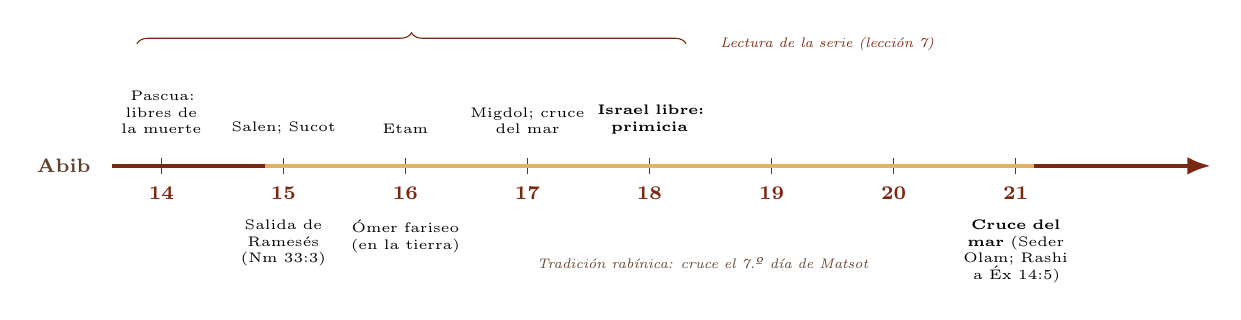
\begin{tikzpicture}[x=1.55cm,font=\scriptsize]
 \draw[line width=1.4pt,tierraroja,-{Latex[length=3mm]}] (-0.4,0) -- (8.6,0);
 \foreach \d [count=\i from 0] in {14,15,16,17,18,19,20,21}{
   \draw[tierraroja] (\i,-0.1) -- (\i,0.1); \node[font=\scriptsize\bfseries,text=tierraroja] at (\i,-0.35) {\d};}
 \node[anchor=east,font=\scriptsize\bfseries,text=sepia] at (-0.5,0) {Abib};
 % lectura de la serie (arriba)
 \foreach \i/\t in {0/{Pascua: libres de la muerte}, 1/{Salen; Sucot}, 2/{Etam}, 3/{Migdol; cruce del mar}, 4/{\textbf{Israel libre: primicia}}}{
   \node[above=8pt,text width=1.45cm,align=center,font=\tiny] at (\i,0) {\t};}
 \node[anchor=west,font=\tiny\itshape,text=tierraroja] at (4.5,1.55) {Lectura de la serie (lección 7)};
 \draw[decorate,decoration={brace,amplitude=4pt},tierraroja] (-0.2,1.55) -- (4.3,1.55);
 % lectura rabinica (abajo)
 \node[below=16pt,text width=1.45cm,align=center,font=\tiny] at (1,0) {Salida de Ramesés (Nm 33:3)};
 \node[below=16pt,text width=1.55cm,align=center,font=\tiny] at (7,0) {\textbf{Cruce del mar} (Seder Olam; Rashi a Éx 14:5)};
 \node[below=16pt,text width=1.45cm,align=center,font=\tiny] at (2,0) {Ómer fariseo (en la tierra)};
 \node[anchor=west,font=\tiny\itshape,text=sepia] at (3.0,-1.25) {Tradición rabínica: cruce el 7.º día de Matsot};
 \fill[mostaza!80] (0.85,0.03) rectangle (7.15,-0.03);
\end{tikzpicture}\par
{\footnotesize\color{sepia}\textit{Figura 9.} Del 14 al 21 de Abib: el itinerario de la serie y la fecha rabínica del cruce. \textit{Nota.} Elaboración propia sobre el documento de referencia, Nm 33:3--8 y Seder Olam Rabá 5.}
\end{center}

\begin{nota}[Precisión: la cronología del cruce y del éxodo]
El documento sitúa el cruce del mar el tercer día de la marcha (17 de Abib) y presenta el 18 como el día de Israel libre, primicia de las naciones. La Biblia no da la fecha del cruce: Nm 33:5--8 enumera Sucot, Etam y Pi-hahirot sin contar los días de cada etapa, y Éx 13:20--14:2 menciona un rodeo. La tradición rabínica lo sitúa el 21 de Nisán, el séptimo día de los Ázimos (Seder Olam Rabá 5; Rashi a Éx 14:5), y por eso la lectura de la Torá de ese día es el Cántico del Mar (Éx 15). En cuanto al año, la serie fecha el éxodo en 1529 a.\,e.\,c.; la cronología interna de 1~R 6:1 (480 años antes del cuarto año de Salomón) da ca. 1446 a.\,e.\,c. (fecha temprana), y muchos historiadores proponen ca. 1260 a.\,e.\,c. (fecha tardía). Además, Éx 19:5--6 se pronuncia en el Sinaí ``en el mes tercero'' (Éx 19:1), y el Ómer mismo no se ofreció en el desierto, pues es ley ``cuando hayáis entrado en la tierra'' (Lv 23:10). La lectura de la serie es, por tanto, tipológica: el Ómer, ofrecido en la tierra durante los Ázimos, \emph{recuerda} la consagración de Israel como primicia, que comenzó con la salida y el cruce. Jer 2:2--3 es el texto que mejor la sostiene.
\end{nota}

\subsection{Figura: el Ómer y Cristo recibido a la diestra}
La lección 11 da la segunda mitad de la tesis. Siguiendo la ``constante simbólica'' de las fiestas (el cordero = Cristo sacrificado; la masa sin levadura = la iglesia liberada del pecado), el documento concluye:

\begin{cita}Siguiendo esta constante simbólica, señalada en las Escrituras, resulta claro, que el ``Omer de la Ofrenda Mecida'', incuestionablemente representaba al Señor Jesús, en una nueva función tras ser recibido en el cielo a la diestra de Dios, el Padre.\fuente{(Documento de referencia, lección 11)}\end{cita}

La formulación merece atención, porque el documento no identifica el Ómer con la resurrección como hecho, sino con Cristo ``en una nueva función'' después de ser recibido a la diestra del Padre. Es una lectura sacerdotal. El Ómer era \emph{presentado} ``delante de \SENOR'' por el sacerdote ``para que seáis aceptos''; Cristo resucitado se presenta ante el Padre y, aceptado, hace aceptos a los suyos. Hebreos expresa la misma idea sin hablar del Ómer: Cristo entró ``en el cielo mismo para presentarse ahora por nosotros ante Dios'' (He 9:24). La lección 8 conecta esa figura con los textos de Pablo: ``la primicia de los resucitados para vida eterna'' (Col 1:18; 1~Co 15:22--23; el documento escribe ``Colosenses 2:18'' por Col 1:18).

\begin{nota}[Precisión: la autoría de Hebreos]
El documento de referencia atribuye Hebreos al apóstol Pablo, y en su voz se mantiene esa atribución al exponerlo. La autoría de la carta es discutida desde la Antigüedad (Orígenes: ``quién escribió la epístola, solo Dios lo sabe''); los comentarios modernos la tratan como anónima (Attridge, 1989; Lane, 1991). El argumento de este capítulo descansa en el texto canónico, no en la autoría.
\end{nota}

Esta lectura tiene una consecuencia para la fecha. Si el Ómer figura la presentación de Cristo ante el Padre, el texto evangélico que la enmarca es Jn 20:17, el mismo que cita el folleto de la Iglesia de Dios Unida (2011): ``No me toques, porque aún no he subido a mi Padre'' (§8.3). En la cronología que adopta la serie (§8.2), esa presentación ocurre el domingo 18 de Abib, ``el día siguiente del sábado'' y día del Ómer. La serie cuenta además los días de Pentecostés desde ese momento: el Espíritu fue derramado ``10 días después del retorno del Señor Jesús a la diestra de su Padre'' (lección 11), es decir, los cuarenta días de Hch 1:3 más diez, dentro de los cincuenta de la cuenta del Ómer.

\subsection{Vigencia: ``cumplido su objetivo''}
La tercera parte de la tesis es la más característica del documento. Mientras sostiene que las fiestas de Levítico 23 siguen vigentes para la iglesia (Lc 23:56; Hch 2:1; 12:3; 20:6, 16; 1~Co 5:8; 16:8; Col 2:16--17), afirma del Ómer:

\begin{cita}Obviamente que cumplido su objetivo la ceremonia del Omer de la ofrenda encendida, dejó de tener vigencia para la Iglesia del Nuevo Pacto.\fuente{(Documento de referencia, lección 8)}\end{cita}

La posición es coherente con el propio marco del documento. El Ómer ``no era un día de guardar'': no es \emph{mikrá kódesh} ni día de reposo, y por eso no figura entre las convocaciones que la iglesia apostólica sigue guardando según Hechos. Su contenido era una figura de un hecho único, la presentación del Hijo como primicia, y una vez cumplido ese hecho el gesto que lo anunciaba no se repite, del mismo modo que no se repite el sacrificio. Pentecostés, en cambio, permanece, porque su contenido (los dos panes, la siega del Espíritu) sigue en curso.

\begin{nota}[Precisión: ``estatuto perpetuo'' y el texto del documento]
Lv 23:14 llama al Ómer \emph{juqat olam}, ``estatuto perpetuo''. La serie resuelve la tensión con la categoría de cumplimiento: lo perpetuo es lo que el rito significa, realizado en Cristo, no la repetición del gesto. El judaísmo rabínico, tras la destrucción del Templo (70 e.\,c.), mantuvo la cuenta como memorial y suspendió la ofrenda; otras comunidades celebran hoy un ``día de las primicias'' (Chumney, 1994). En la cita de la lección 8, ``ofrenda encendida'' parece una errata por ``ofrenda mecida'', que es la expresión del resto del documento; la ``ofrenda encendida'' de Lv 23:13 es la \emph{minjá} que acompaña al Ómer.
\end{nota}

\subsection{La lectura de Danilo: las primicias y el diecisiete de Nisán}\label{sec:danilo}
La presentación de Danilo \emph{Los Panes sin Levadura} dedica una parte a las primicias y la integra en su lectura de la semana de Pascua. Lee Lv 23:9--14 con glosas judías: el ómer es una medida de cebada (≈\,3.500\,cm³), y ``el día posterior a Shabat'' es el día posterior al primer día de Pésaj, según la lectura rabínica (§5.2). Describe así la ceremonia: cuando la cebada (y luego el trigo) estaba lista, se tomaba una sola gavilla, ``la gavilla de los primeros frutos'', y el sacerdote la mecía ante Dios ``el día después del sábado'', con las ofrendas prescritas. Su concepto de primicias tiene tres rasgos: son \destacar{siempre lo mejor y lo primero}; son \destacar{santas ante Dios}, como el primogénito de hombre y de bestia (``Conságrame todo primogénito'', Éx 13:2; ``No demorarás la primicia de tu cosecha ni de tu lagar. Me darás el primogénito de tus hijos'', Éx 22:29 [22:28]); y se presentan \destacar{con alabanza}, como en la canasta de Dt 26:1--11.

\paragraph{El diecisiete de Nisán.} Danilo sitúa en el 17 de Nisán varios hitos de la historia bíblica, que leídos juntos forman una cadena de ``vida desde la muerte''. Son cómputos tradicionales, no fechas explícitas del texto, y cada uno se precisa a continuación:

\begin{center}\begin{minipage}{\linewidth}\centering\footnotesize\renewcommand{\arraystretch}{1.15}
\begin{tabular}{@{}L{3.0cm}L{4.4cm}L{7.0cm}@{}}
\toprule
\textbf{Hito} & \textbf{Cómputo de Danilo} & \textbf{Precisión con el texto} \\ \midrule
El arca reposa en el Ararat (Gn 8:4) & ``mes séptimo, a los diecisiete días'', con el calendario civil que empieza en Tishri: el séptimo mes es Nisán & El texto dice ``mes séptimo'' sin nombre. Si se cuenta desde Tishri, es Nisán; si desde Nisán, es Tishri. Los rabinos lo discuten (R. Eliezer y R. Yehoshúa, Talmud de Babilonia, Rosh haShaná 11b; tradición). \\
Israel cruza el mar (Éx 14) & salida el 15 + ``camino de tres días'' (Éx 3:18; 5:3) = 17 & Los ``tres días'' son la petición al faraón, no una fecha del cruce; Éx 14 no da el día. El documento de referencia coincide en el 17; la tradición rabínica da el 21 (Seder Olam 5). \\
Israel come el primer fruto de la tierra (Jos 5:10--12) & ``cumplimiento histórico de Lv 23:9--13'' & Josué dice ``al otro día de la pascua'' (15 según Nm 33:3; 16 según la lectura rabínica) y que el maná cesó ``el día siguiente'' (16 o 17). \\
Amán es derrotado (Est 3--7) & decreto el 13 de Nisán (Est 3:12); ayuno de tres días desde el 13--14 (Est 4:16) & Ester no fecha el ayuno ni la caída de Amán. La tradición rabínica la sitúa el 16, y cuenta que Amán encontró a Mardoqueo enseñando las leyes del ómer (Talmud de Babilonia, Meguilá 16a; tradición; verificar). \\
\bottomrule
\end{tabular}\par
{\footnotesize\color{sepia}\textit{Tabla 5.} El diecisiete de Nisán en la lectura de Danilo. \textit{Nota.} Elaboración propia a partir de la presentación \emph{Los Panes sin Levadura} de Danilo Gómez Correa.}
\end{minipage}\end{center}

La cadena tiene fuerza literaria: el arca que se posa sobre un mundo nuevo, el pueblo que sale vivo del mar, el primer pan de la tierra prometida y el enemigo de los judíos derrotado. Su base cronológica, en cambio, es variable: depende de cómo se cuente el ``mes séptimo'' de Génesis, de cuándo se fije el cruce y de cómo se lean Josué y Ester. Conviene presentarla como lectura tipológica de la serie, apoyada en cómputos tradicionales.

\paragraph{Jesús, la primicia de la cosecha de cebada.} El título de Danilo resume la cristología del tema: Jesús es la primicia de la primera cosecha del año. La presentación reúne los textos del \emph{primogénito}: primogénito de María (Mt 1:23--25), primogénito introducido en el mundo por el Padre (He 1:6), ``el primogénito de toda creación'' (Col 1:15), ``el primogénito de los muertos'' (Ap 1:5), ``el primogénito entre muchos hermanos'' (Ro 8:29), ``primicias de los que durmieron'' (1~Co 15:20, 23), ``el principio de la creación de Dios'' (\grc{ἡ ἀρχὴ τῆς κτίσεως τοῦ θεοῦ}, Ap 3:14) y el que ``en todo tenga la preeminencia'' (Col 1:18). La lista une las dos raíces del campo semántico (§4): \emph{bejor}/\grc{πρωτότοκος} y \emph{reshit}/\grc{ἀρχή}--\grc{ἀπαρχή}. Danilo cierra con 1~Co 15:20--23: ``Cristo, las primicias; luego los que son de Cristo, en su venida''.

\begin{nota}[Precisión textual: Mt 1:25]
La RVR1960 lee en Mt 1:25 ``hasta que dio a luz a su hijo primogénito'', con el texto mayoritario (\grc{τὸν υἱὸν αὐτῆς τὸν πρωτότοκον}). NA28, con el Sinaítico y el Vaticano, lee solo ``un hijo'' (\grc{υἱόν}); el término ``primogénito'' está asegurado en Lc 2:7. El argumento de Danilo no cambia: Jesús es el primogénito de María por Lc 2:7.
\end{nota}

\subsection{La congregación de los primogénitos}
El documento usa He 12:22--24 para su primer período de la iglesia: la ``congregación de los primogénitos que están inscritos en los cielos'' (\grc{ἐκκλησίᾳ πρωτοτόκων ἀπογεγραμμένων ἐν οὐρανοῖς}, He 12:23), que identifica con los fieles desde Adán hasta el pacto con Abraham. La expresión pertenece al campo de las primicias: \grc{πρωτότοκος} traduce \emph{bejor}. Los comentarios suelen entenderla como el pueblo de Dios en su conjunto, inscrito en el cielo como Israel era el ``primogénito'' (Éx 4:22), o como los ángeles (Attridge, 1989; Lane, 1991). La lectura del documento es una tercera opción, propia de su esquema de tres períodos, y se expone aquí como tal.

%===================================================================
\section{La fiesta en Jesús y los apóstoles}

\subsection{``El primer día de la semana''}
Los cuatro evangelios sitúan la tumba vacía ``el primer día de la semana'': \grc{εἰς μίαν σαββάτων} (Mt 28:1), \grc{τῇ μιᾷ τῶν σαββάτων} (Mc 16:2; Lc 24:1; Jn 20:1, 19). La expresión griega dice literalmente ``el uno de los sábados'': \grc{σάββατα} designa la semana, igual que \emph{shabatot} en Lv 23:15. Si el ``sábado'' de Lv 23:11 es el sábado semanal, el Ómer caía siempre ``el primer día de la semana'', el mismo día de la resurrección. Si es el 15 de Nisán, la coincidencia depende del año. El cálculo exige elegir primero una cronología de la Pasión:

\begin{center}\begin{minipage}{\linewidth}\centering\footnotesize\renewcommand{\arraystretch}{1.15}
\begin{tabular}{@{}L{3.6cm}L{3.3cm}L{3.5cm}L{3.9cm}@{}}
\toprule
\textbf{Cronología de la Pasión} & \textbf{Domingo de la resurrección} & \textbf{Ómer fariseo (16)} & \textbf{Ómer saduceo (domingo)} \\ \midrule
Juan: crucifixión el viernes 14 (Jn 18:28; 19:14, 31) & 16 de Nisán & domingo 16: \textbf{coincide} & domingo 16: \textbf{coincide} \\
Sinópticos: Cena pascual; crucifixión el viernes 15 & 17 de Nisán & sábado 16: Jesús en la tumba & domingo 17: \textbf{coincide} \\
\textbf{\color{tierraroja}Lectura de la serie (adoptada):} crucifixión el miércoles 14 (Mt 12:40); resurrección al cerrarse el sábado 17 (Mt 28:1) & \textbf{domingo 18}: tumba vacía y día del Ómer; Cristo se presenta ante el Padre (Jn 20:17) & viernes 16 & \textbf{domingo 18: coincide} con el 18 de Abib, Israel primicia (documento de referencia) \\
\bottomrule
\end{tabular}\par
{\footnotesize\color{sepia}\textit{Tabla 4.} El Ómer y la resurrección según cada cronología. \textit{Nota.} Cálculo propio. La tercera fila es la cronología que adopta la serie (§8.2); armoniza el 18 de Abib del documento de referencia, el 17 de Nisán de la presentación de Danilo y la lectura de \emph{mimojorat hashabat} como sábado semanal. En el calendario de Qumrán (Ómer el 26) no hay coincidencia en ningún caso.}
\end{minipage}\end{center}

\begin{nota}[Precisión: cálculo cronológico]
La tabla es un cálculo, no un dato del texto. La cronología joánica, preferida por muchos historiadores, hace caer el 15 de Nisán en sábado, ``aquel día de reposo'' que ``era de gran solemnidad'' (Jn 19:31); en ese caso las lecturas farisea y saducea dan el mismo domingo 16, y la ofrenda del Ómer en el Templo coincidió con la mañana de la resurrección. Los años propuestos con más frecuencia (30 o 33 e.\,c.) admiten esa configuración según los cálculos astronómicos, con el margen de un calendario de observación. La tercera fila, que adopta la serie, coincide con la posición de varias iglesias de tradición sabatista, que leen ``tres días y tres noches'' (Mt 12:40) como setenta y dos horas; en ella el domingo cae el 18 de Abib, la misma fecha que el documento de referencia asigna a Israel ``primicia de las naciones''.
\end{nota}

\subsection{``Tres días y tres noches'': la cronología de la serie}
La presentación de Danilo sobre los Ázimos aporta los argumentos con que la serie fija su cronología de la Pasión. Parten de la señal de Jonás:

\begin{cita}Porque como estuvo Jonás en el vientre del gran pez tres días y tres noches, así estará el Hijo del Hombre en el corazón de la tierra tres días y tres noches.\fuente{(Mt 12:40)}\end{cita}

Danilo reúne las ``sombras proféticas'' del tercer día en el Tanaj: Abraham ve el lugar del sacrificio ``al tercer día'' (Gn 22:4); Moisés pide al faraón ``camino de tres días'' para sacrificar (Éx 3:18; 5:3; 8:27 [8:23]); Ester ayuna ``tres días, noche y día'' y ``al tercer día'' se presenta ante el rey (Est 4:16; 5:1); Jonás está tres días y tres noches en el pez (Jon 1:17 [2:1]). Jesús anuncia que resucitará ``al tercer día'' (Mt 16:21) y lo explica con las Escrituras (Lc 24:44--46). De ahí concluye que, crucificado el 14 de Nisán, Jesús resucitó en el 17 de Nisán, que ese año fue sábado semanal dentro de la semana de Pascua; las mujeres encontraron la tumba vacía ``el primer día de la semana'' (Mc 16:1--6). El 17 es, en su lectura, el día en que, según su cómputo, Israel cruzó el mar y comió el primer fruto de la tierra (§7.5). La serie integra este dato con el 18 de Abib del documento de referencia y con la ley del Ómer:

\begin{tcolorbox}[enhanced,unbreakable,colback=papiro,colframe=tierraroja,boxrule=1pt,arc=3pt,fonttitle=\bfseries\small,coltitle=papiro,colbacktitle=tierraroja,fontupper=\small,title={Lectura de la serie: la cronología adoptada}]
\begin{enumerate}\setlength{\itemsep}{1pt}
\item \textbf{14 de Abib, miércoles} (en esta reconstrucción): Cristo, nuestra pascua, muere y es sepultado antes de la puesta del sol (1~Co 5:7; Jn 19:31, 42).
\item \textbf{15 de Abib, jueves}: primer día de los Ázimos, día de reposo festivo: el ``gran día'' de Jn 19:31.
\item \textbf{17 de Abib, sábado semanal}: al cerrarse el sábado se cumplen los ``tres días y tres noches'' (Mt 12:40). Mateo sitúa la escena ``pasado el día de reposo'' (\grc{ὀψὲ δὲ σαββάτων}, Mt 28:1). Es el 17 de la presentación de Danilo.
\item \textbf{18 de Abib, domingo}: ``el día siguiente del sábado'' (\emph{mimojorat hashabat}, leído como sábado semanal) y ``el primer día de la semana'' en que se constata la tumba vacía (Mc 16:2; Jn 20:1). Es el día del Ómer: Cristo, ``primicias de los que durmieron'' (1~Co 15:20), aún no ha subido al Padre por la mañana (Jn 20:17) y se presenta ante él como la gavilla ``delante de \SENOR{}\ldots{} para que seáis aceptos'' (Lv 23:11). La fecha coincide con el 18 de Abib que el documento de referencia asigna a Israel, primicia de las naciones.
\end{enumerate}
\emph{Fundamentos}: la lectura literal de Mt 12:40; \grc{ὀψὲ σαββάτων} en Mt 28:1; la distinción entre el momento de la resurrección (que ningún evangelio narra) y el hallazgo de la tumba vacía (Mc 16:2); la lectura de \emph{shabat} en Lv 23:11, 15--16 como sábado semanal (§5.3); y la coherencia de la cadena memorial--figura de la serie (§7).
\end{tcolorbox}

\begin{nota}[Precisión: alternativas que se mantienen en la discusión académica]
(1) La cronología tradicional, viernes--domingo, se apoya en el cómputo inclusivo hebreo: Ester ayuna ``tres días, noche y día'' (Est 4:16) y entra ante el rey ``al tercer día'' (5:1), y los evangelios alternan ``después de tres días'' y ``al tercer día'' (Mt 27:63--64; Mc 8:31; Lc 24:21). (2) La lectura farisea fija el Ómer el 16 de Nisán, cualquiera sea el día de la semana (§5.2); con la cronología joánica el 16 cae en domingo. (3) El calendario de los años 30 y 33 e.\,c. es discutido: depende de la observación de la luna nueva y de la intercalación, y los cálculos astronómicos no deciden por sí solos en qué día de la semana cayó el 14 de Nisán. (4) Jn 19:31 llama a ese sábado ``de gran solemnidad''; la lectura tradicional lo entiende como sábado semanal coincidente con el 15, y la de la serie como el día festivo del 15, distinto del sábado semanal. (5) Mc 16:9, que dice ``habiendo, pues, resucitado Jesús por la mañana, el primer día de la semana'', pertenece al final largo de Marcos (16:9--20), ausente en los códices Sinaítico y Vaticano; su puntuación se discute (``por la mañana'' puede ir con ``apareció''). La serie no deja la cuestión abierta, pero estas alternativas forman parte del estado de la discusión.
\end{nota}

\subsection{``No me toques, porque aún no he subido a mi Padre''}
El encuentro de Jesús con María Magdalena, la mañana del primer día, incluye una frase enigmática:

\begin{cita}Jesús le dijo: No me toques, porque aún no he subido a mi Padre; mas ve a mis hermanos, y diles: Subo a mi Padre y a vuestro Padre, a mi Dios y a vuestro Dios.\fuente{(Jn 20:17)}\end{cita}

El griego \grc{μή μου ἅπτου} es un imperativo presente con negación, que suele indicar el cese de una acción en curso: ``deja de retenerme'', ``no te aferres a mí'' (Brown, 1970; Keener, 2003). Para la mayoría de los comentaristas, Jesús explica que su presencia resucitada no es un regreso a la situación anterior: la relación nueva vendrá después de su ``subida'' al Padre y del don del Espíritu (Jn 20:22). Algunos intérpretes leen el versículo tipológicamente: Cristo, primicia, debía presentarse primero ante el Padre, como la gavilla ``delante de \SENOR'', antes de ser tocado; ocho días después invita a Tomás a tocarlo (Jn 20:26--27), y Mateo dice que las mujeres ``abrazaron sus pies'' (Mt 28:9). Esta es la lectura de la Iglesia de Dios Unida (2011) y la que mejor se ajusta a la fórmula del documento de referencia (``recibido\ldots{} a la diestra''). Es una lectura tipológica posible; el texto de Juan no menciona el Ómer.

\subsection{Los santos que se levantaron}
Mateo añade un detalle único a la muerte de Jesús:

\begin{cita}\ldots{} y la tierra tembló, y las rocas se partieron; y se abrieron los sepulcros, y muchos cuerpos de santos que habían dormido, se levantaron; y saliendo de los sepulcros, después de la resurrección de él, vinieron a la santa ciudad, y aparecieron a muchos.\fuente{(Mt 27:51--53)}\end{cita}

La frase ``que habían dormido'' es \grc{τῶν κεκοιμημένων ἁγίων}, el mismo participio que Pablo usa en 1~Co 15:20 (\grc{ἀπαρχὴ τῶν κεκοιμημένων}). Mateo subraya que salieron ``después de la resurrección de él'': Cristo va primero. Algunos autores ven en estos santos la ``gavilla'' que acompaña a la primicia (Chumney, 1994); otros, una señal apocalíptica del inicio de la resurrección de los muertos (cf. Ez 37:12--13; Dn 12:2). El texto no explica más, y conviene no cargarlo con detalles que no da.

\subsection{Pablo: ``Cristo, primicias de los que durmieron''}
El centro neotestamentario del tema es 1 Corintios 15. Contra quienes decían que ``no hay resurrección de muertos'' (15:12), Pablo afirma el hecho y su orden:

\begin{cita}Mas ahora Cristo ha resucitado de los muertos; primicias de los que durmieron es hecho. Porque por cuanto la muerte entró por un hombre, también por un hombre la resurrección de los muertos. Porque así como en Adán todos mueren, también en Cristo todos serán vivificados. Pero cada uno en su debido orden: Cristo, las primicias; luego los que son de Cristo, en su venida. Luego el fin, cuando entregue el reino al Dios y Padre, cuando haya suprimido todo dominio, toda autoridad y potencia.\fuente{(1~Co 15:20--24)}\end{cita}

Pablo lee aquí la Escritura de Israel como trama que culmina en Cristo (Hays, 1989): la lógica es la de Ro 11:16: la primicia es la primera parte de \emph{la misma} cosecha y garantiza el resto. Si Cristo es la gavilla, la siega de ``los que durmieron'' ya empezó. La palabra \grc{τάγμα} (``orden'', v. 23) es un término militar: el rango o la formación de una tropa que avanza en orden. Pablo enumera tres momentos: \grc{ἀπαρχὴ Χριστός}, \grc{ἔπειτα οἱ τοῦ Χριστοῦ ἐν τῇ παρουσίᾳ αὐτοῦ}, \grc{εἶτα τὸ τέλος}.

\begin{center}
\begin{tikzpicture}[font=\scriptsize,
  s/.style={draw=tierraroja,line width=0.9pt,fill=papiro,rounded corners=3pt,text width=3.25cm,align=center,inner sep=5pt,minimum height=2.2cm},
  d/.style={draw=sepia!70,dashed,line width=0.6pt,fill=white,rounded corners=3pt,text width=2.7cm,align=center,inner sep=4pt,minimum height=2.2cm,font=\tiny}]
 \node[s] (a) at (0,0) {\textbf{\color{tierraroja}1. \grc{ἀπαρχὴ Χριστός}}\\[2pt]``Cristo, las primicias''\\ resurrección (15:20, 23)\\[2pt]\textit{la gavilla mecida}};
 \node[d] (p) at (3.85,0) {\textit{Entre ambas:}\\ ``las primicias del Espíritu'' (Ro 8:23; cf. Stg 1:18)\\[2pt]\textit{Pentecostés}};
 \node[s] (b) at (7.7,0) {\textbf{\color{tierraroja}2. \grc{οἱ τοῦ Χριστοῦ}}\\[2pt]``los que son de Cristo, en su venida''\\ (15:23; ``a la final trompeta'', 15:52)\\[2pt]\textit{Trompetas}};
 \node[s] (c) at (11.55,0) {\textbf{\color{tierraroja}3. \grc{τὸ τέλος}}\\[2pt]``luego el fin'': el reino entregado al Padre; la muerte destruida (15:24--28)\\[2pt]\textit{Octavo día}};
 \draw[-{Latex[length=2.5mm]},line width=1.2pt,mostaza] (a) -- (p);
 \draw[-{Latex[length=2.5mm]},line width=1.2pt,mostaza] (p) -- (b);
 \draw[-{Latex[length=2.5mm]},line width=1.2pt,mostaza] (b) -- (c);
 \node[font=\tiny,text=sepia,text width=14.5cm,align=center] at (5.8,-1.75) {Arriba: el texto de Pablo (\grc{ἀπαρχή} -- \grc{ἔπειτα} -- \grc{εἶτα}). En cursiva: la correspondencia con las fiestas según la lectura de la serie. El recuadro discontinuo no está en 1~Co 15.};
\end{tikzpicture}\par
{\footnotesize\color{sepia}\textit{Figura 10.} 1~Co 15:20--28 como secuencia. \textit{Nota.} Elaboración propia sobre NA28 y el documento de referencia (cuadro de las fiestas, \emph{GUIA} de la serie).}
\end{center}

La serie lee este orden como la secuencia de las fiestas: la primicia (el Ómer, Cristo), la venida ``a la final trompeta'' (1~Co 15:52; Yom Teruá) y ``luego el fin'', que el documento asocia al octavo día y al juicio final (Ap 20:7--15). Es una lectura coherente con el vocabulario de Pablo, que en la misma carta llama a Cristo ``nuestra pascua'' (1~Co 5:7), menciona Pentecostés (1~Co 16:8) y aquí la primicia: el calendario de la primavera atraviesa la carta. Pablo no nombra las fiestas en 1~Co 15:20--28, y por eso la correspondencia es tipológica. Lo que Pablo sí dice, con toda claridad, es que la resurrección tiene un orden y que Cristo va primero.

\begin{nota}[Precisión: 1 Corintios y el calendario]
Fee (1987) y otros comentaristas observan que 1~Corintios se escribe en Éfeso antes de Pentecostés (16:8) y que sus imágenes pascuales (5:7--8) podrían reflejar la estación en que Pablo escribe. Es una conjetura razonable, no un dato. La palabra \grc{ἀπαρχή}, en cambio, sí tiene trasfondo cultual seguro: es el término de la LXX para la gavilla de Lv 23:10.
\end{nota}

\subsection{Las primicias en las demás cartas y en Apocalipsis}
El resto del Nuevo Testamento extiende la imagen de Cristo a los suyos. Los creyentes tienen ``las primicias del Espíritu'' y esperan ``la redención de nuestro cuerpo'' (Ro 8:23): el Espíritu es la primera gavilla de una cosecha que es la resurrección corporal. Santiago, en un lenguaje que recuerda la creación, dice que Dios ``de su voluntad, nos hizo nacer por la palabra de verdad, para que seamos primicias de sus criaturas'' (Stg 1:18): la iglesia es la primera parte de una creación renovada. Los primeros convertidos de una región son su primicia (Ro 16:5; 1~Co 16:15). Apocalipsis llama a los 144\,000 ``primicias para Dios y para el Cordero'' (Ap 14:4), y a continuación describe dos siegas, la del grano y la de la vid (Ap 14:14--20): la primicia precede, como en Levítico, a la cosecha completa. Colosenses une las dos palabras del campo: Cristo es \grc{ἀρχή} y \grc{πρωτότοκος ἐκ τῶν νεκρῶν}, ``el principio, el primogénito de entre los muertos'' (Col 1:18), donde \grc{ἀρχή} podría ser eco de \emph{reshit}.

\begin{nota}[Precisión: cartas de autoría discutida]
Parte de la crítica considera que Colosenses y 2~Tesalonicenses fueron escritas por discípulos de Pablo. El argumento de este capítulo se apoya en las cartas indiscutidas (1~Co 15:20--23; Ro 8:23; 11:16; 16:5), y Colosenses y 2~Tesalonicenses solo confirman el uso.
\end{nota}

%===================================================================
\section{La fiesta en la tradición judía}

\subsection{La cuenta del ómer}
Tras la destrucción del Templo, el judaísmo rabínico conservó la cuenta y suspendió la ofrenda. La práctica de la \heb{סְפִירַת הָעֹמֶר} (\emph{sefirat haómer}) consiste en contar en voz alta, cada noche desde el 16 de Nisán, los días y las semanas transcurridas, precedidos de una bendición: ``hoy es el día treinta y tres, que son cuatro semanas y cinco días del ómer''. El Talmud discute si el precepto de contar sigue vigente sin Templo o es solo un memorial (Talmud de Babilonia, Menajot 66a; tradición). Con el tiempo, el período adquirió un tono de semiduelo, que la tradición explica por la muerte de los discípulos de rabí Aquiba (Yevamot 62b), y el día 33 de la cuenta, \emph{Lag baÓmer}, se volvió una jornada de alegría. La cábala medieval asignó a cada día una combinación de las \emph{sefirot}. Todo ello es desarrollo posterior a la Biblia y al Nuevo Testamento.

\subsection{Shavuot como fiesta de la Torá}
La fecha fija del 6 de Siván, que resulta del cómputo fariseo, permitió a la tradición rabínica asociar Shavuot con la entrega de la Torá en el Sinaí, que Éx 19:1 sitúa ``en el mes tercero''. El Talmud discute si la Torá se dio el 6 o el 7 de Siván (Shabat 86b). La serie hace la misma asociación por otra vía: Pentecostés es memorial de ``la manifestación del Espíritu de Dios en el monte Sinaí y la data de la Ley''. En ese esquema, la cuenta del Ómer va de la liberación a la ley: Israel sale de Egipto para servir a Dios en el monte (Éx 3:12).

\subsection{Caraítas, samaritanos y cristianos}
Los caraítas, desde Anán ben David (siglo \textsc{viii}), rechazaron la interpretación rabínica y cuentan desde el domingo dentro de los Ázimos; también los samaritanos celebran Shavuot siempre en domingo. Entre los cristianos, el calendario litúrgico calcula Pentecostés a partir del domingo de Pascua de Resurrección, de modo que cae siempre en domingo: la coincidencia formal con la lectura saducea es evidente, aunque el cómputo cristiano no se derivó directamente de esa controversia. Algunas comunidades judeomesiánicas y evangélicas celebran hoy un \emph{Yom haBikurim} como fiesta de la resurrección (Chumney, 1994); el documento de referencia, en cambio, considera cumplido el Ómer.

%===================================================================
\section{Discusión de interpretaciones}

\subsection{¿Qué sábado?}
La fecha del Ómer es el debate más antiguo sobre Levítico 23 del que hay registro. La lectura del 16 de Nisán tiene a su favor la antigüedad de sus testigos (LXX, Filón, Josefo) y la coherencia con un calendario de fechas fijas; la del domingo, la lectura más natural de \emph{shabat} y de las ``siete \emph{shabatot}''; la de Qumrán, la coherencia de un calendario solar que buscaba fechas y días de la semana fijos (VanderKam, 1998). Milgrom (2001) y Levine (1989) exponen el debate en detalle; Wenham (1979) y Hartley (1992) muestran que el texto, por sí solo, admite más de una lectura. Para un estudio que sigue el principio de que la Biblia interpreta la Biblia, la conclusión prudente es doble: la Escritura no da un número para el Ómer, y su silencio fue leído de modos distintos por grupos que querían obedecerla. La consecuencia práctica (en qué día se guarda Pentecostés) depende de una decisión interpretativa que conviene hacer explícita.

\subsection{¿Mecer o elevar?}
La tradición rabínica entiende la \emph{tenufá} como un movimiento en las cuatro direcciones y hacia arriba y abajo (Misná Menajot 5:6; Talmud de Babilonia, Menajot 62a), y la RVR1960 sigue esa imagen (``mecer''). Milgrom (1991) defiende el sentido de ``elevación'', un gesto de transferencia al dominio divino, apoyado en el uso para los levitas (Nm 8:11--21) y en traducciones de la LXX como \grc{ἀνοίσει} (Lv 23:11). Gane (2004) resume las dos posiciones. Para la teología del rito la diferencia es menor: en ambos casos la gavilla sale del ámbito del agricultor y pasa al de Dios, ``delante de \SENOR''.

\subsection{¿Resurrección, presentación o anticipo?}
Tres énfasis se distinguen en la lectura cristiana del Ómer. (1) La mayoría de los comentarios de 1 Corintios entiende \grc{ἀπαρχή} como \emph{anticipo y garantía}: la primera parte de la cosecha es prenda de la cosecha entera (Fee, 1987; Thiselton, 2000; Dunn, 1998). El énfasis está en la solidaridad entre Cristo y los suyos, no en el calendario. (2) Otros autores subrayan la \emph{coincidencia de fecha} entre la resurrección y la ofrenda de la gavilla, y ven en ella un cumplimiento del calendario (Chumney, 1994; Iglesia de Dios Unida, 2011). (3) El documento de referencia de la serie, con la cronología del §8.2, pone el acento en la \emph{presentación}: el Ómer representa a Cristo ``en una nueva función tras ser recibido en el cielo a la diestra de Dios''. Las tres lecturas no se excluyen; difieren en qué aspecto del rito consideran central: la gavilla como primera parte, la fecha, o el gesto sacerdotal ``delante de \SENOR{}\ldots{} para que seáis aceptos''. La tercera es la que más aprovecha el texto de Lv 23:11.

\subsection{¿Hay un intervalo entre la venida y el fin?}
En 1~Co 15:23--24, \grc{ἔπειτα} y \grc{εἶτα} pueden indicar sucesión inmediata o con intervalo. Las lecturas premilenaristas ven entre la venida (\grc{παρουσία}) y ``el fin'' el reino de Ap 20:4--6; la serie lo identifica con Sukkot y el Milenio, y el fin con el octavo día. Fee (1987) y Thiselton (2000) sostienen que Pablo no piensa aquí en un reino intermedio y que ``el fin'' sigue a la venida. Wright (2003) subraya que el argumento de Pablo se centra en la derrota de la muerte, ``el postrer enemigo'' (15:26). El texto de Pablo no resuelve por sí solo la cuestión; la lectura de la serie se apoya en Apocalipsis 20.

%===================================================================
\section{Síntesis}

\begin{tcolorbox}[enhanced,unbreakable,colback=papiro,colframe=tierraroja,boxrule=1pt,arc=3pt,title={\bfseries El Ómer de las primicias},coltitle=papiro,colbacktitle=tierraroja]
El Ómer es la primera gavilla de la siega de la cebada, presentada por el sacerdote ``delante de \SENOR{}'' el día siguiente del sábado de la semana de los Ázimos, ``para que seáis aceptos'' (Lv 23:10--11). No es convocación santa, pero libera la cosecha nueva (23:14) y abre la cuenta de cincuenta días que termina en Pentecostés (23:15--16). Expresa la ley que recorre la Escritura: \destacar{lo primero pertenece a Dios y consagra el resto} (Gn 4:4; Éx 23:19; Ro 11:16). Israel fue llamado ``primicias de sus nuevos frutos'' (Jer 2:3) desde su juventud en el desierto; Cristo resucitado es ``primicias de los que durmieron'' (1~Co 15:20): según la cronología de la serie, resucitó al cerrarse el sábado 17 y se presentó ante el Padre a favor de los suyos el 18 de Abib, el día siguiente del sábado, día del Ómer; la iglesia es ``primicias de sus criaturas'' (Stg 1:18) y espera, en orden, la cosecha completa: ``Cristo, las primicias; luego los que son de Cristo, en su venida; luego el fin'' (1~Co 15:23--24).
\end{tcolorbox}

\begin{center}\begin{minipage}{\linewidth}\centering\footnotesize\renewcommand{\arraystretch}{1.15}
\begin{tabular}{@{}L{3.2cm}L{11.2cm}@{}}
\toprule
\textbf{Lectura} & \textbf{Aporte al estudio del Ómer} \\ \midrule
Histórica & la cebada madura en Abib (Éx 9:31); Gilgal marca el paso del maná al fruto de la tierra (Jos 5:10--12); Josefo y Filón fijan el rito el 16 de Nisán; la Misná conserva la ceremonia y la polémica con los boetusianos. \\
Filológica & \emph{reshit} (lo primero y lo mejor), \emph{bikurim} (lo primero maduro, raíz de \emph{bejor}), \emph{terumá}, \emph{tenufá}, \emph{lirtsonjem}; la LXX \grc{ἀπαρχή} es el puente directo a 1~Co 15:20. \\
Textual & \emph{mimojorat hashabat} admite tres lecturas (16 de Nisán, domingo en los Ázimos, domingo 26) con consecuencias para Shavuot; la LXX interpreta Lv 23:11; variantes en 2~Ts 2:13, Ro 16:5, Lc 6:1. \\
Literaria & Lv 23:9--22 es una sola unidad: el Ómer mira a Pentecostés; la cuenta es miniatura del jubileo (Lv 25:8); el patrón ``lo primero para Dios'' va de Abel a Apocalipsis. \\
De la serie & memorial de Israel, primicia de las naciones (Éx 19:5--6; Jer 2:3); figura de Cristo recibido a la diestra; rito cumplido que dejó de tener vigencia; el 17 de Nisán y ``Jesús, primicia de la cebada'' (Danilo). \\
Neotestamentaria & cronología de la serie: 14 (crucifixión), 17 (resurrección al cerrarse el sábado), 18 (Ómer y presentación ante el Padre); Jn 20:17 y Mt 27:52--53 como posibles ecos; 1~Co 15:20--28 como orden de la resurrección. \\
\bottomrule
\end{tabular}\par
{\footnotesize\color{sepia}\textit{Tabla 6.} Síntesis: cada lectura y su aporte. \textit{Nota.} Elaboración propia.}
\end{minipage}\end{center}

%===================================================================
\section{Para la reflexión}

\begin{enumerate}
\item El agricultor israelita no comía pan nuevo antes de entregar la gavilla (Lv 23:14). ¿Qué ``primera gavilla'' de su tiempo, sus ingresos o sus decisiones entrega usted antes de disponer del resto, y cuál suele quedar para el final (Pr 3:9--10)?
\item Lv 23:11 dice que la gavilla se mecía ``para que seáis aceptos''. ¿Qué cambia en la vida del creyente saber que su aceptación ante Dios descansa en una primicia presentada por otro (He 9:24; Ef 1:6)?
\item Jeremías recuerda que Israel fue ``primicias'' cuando seguía a Dios ``en tierra no sembrada'' (Jer 2:2--3). ¿Qué rasgos de esa ``juventud'' en el desierto (dependencia, fidelidad, primer amor) ha perdido o conserva su comunidad?
\item Pablo usa la primicia para dar orden a la esperanza (1~Co 15:23). ¿Cómo afecta su manera de enfrentar la muerte de alguien cercano saber que la siega ya empezó con Cristo?
\item El debate sobre ``el día siguiente del sábado'' muestra que lectores fieles de la misma Escritura llegaron a conclusiones distintas. ¿Cómo distinguir, en el estudio de las fiestas, lo que el texto dice de lo que nuestra tradición decide?
\end{enumerate}

%===================================================================
\section*{Glosario}\markboth{Glosario}{}
\begin{description}\small
\item[Abib] (\heb{אָבִיב}). Cebada en espiga, con el grano formado (Éx 9:31); nombre del primer mes, ``mes de la espiga'' (Éx 13:4), llamado Nisán después del exilio.
\item[Aparjé] (\grc{ἀπαρχή}). ``Primicia''; en la LXX traduce \emph{reshit} y \emph{terumá}; en el NT, Cristo resucitado (1~Co 15:20), el Espíritu (Ro 8:23), la iglesia (Stg 1:18).
\item[Bejor] (\heb{בְּכוֹר}). Primogénito; de la raíz \emph{bkr}, ``madurar primero''. Israel es ``mi primogénito'' (Éx 4:22).
\item[Bikurim] (\heb{בִּכּוּרִים}). Los primeros frutos maduros; Shavuot es \emph{yom habikurim} (Nm 28:26); en la Misná, la canasta de Dt 26.
\item[Boetusianos] (\heb{בַּיְתוֹסִים}). Grupo sacerdotal emparentado con los saduceos; según la Misná, contaban el Ómer desde el domingo dentro de los Ázimos (Menajot 10:3).
\item[Drágma] (\grc{δράγμα}). ``Puñado, gavilla''; traducción de la LXX para \emph{ómer} en Lv 23:10.
\item[Lirtsonjem] (\heb{לִרְצֹנְכֶם}). ``Para vuestra aceptación'', ``para que seáis aceptos'' (Lv 23:11); de \emph{ratsón}.
\item[Mimojorat hashabat] (\heb{מִמָּחֳרַת הַשַּׁבָּת}). ``El día siguiente del sábado'' (Lv 23:11, 15, 16); fórmula cuyo sentido divide a fariseos, saduceos y Qumrán.
\item[Minjá] (\heb{מִנְחָה}). Ofrenda vegetal de harina con aceite; con el Ómer, de dos décimas de efa (Lv 23:13).
\item[Ómer] (\heb{עֹמֶר}). Medida de áridos, la décima parte de un efa (Éx 16:36); gavilla de espigas (Rut 2:7; Lv 23:10).
\item[Prōtótokos] (\grc{πρωτότοκος}). ``Primogénito''; Cristo, ``el primogénito de entre los muertos'' (Col 1:18); la ``congregación de los primogénitos'' (He 12:23).
\item[Reshit] (\heb{רֵאשִׁית}). Principio; lo primero y lo mejor de algo; las primicias de la siega (Lv 23:10) y de los frutos (Pr 3:9).
\item[Sefirat haómer] (\heb{סְפִירַת הָעֹמֶר}). La cuenta rabínica de los cuarenta y nueve días desde el 16 de Nisán hasta Shavuot (tradición).
\item[Tenufá] (\heb{תְּנוּפָה}). Ofrenda ``mecida'' o ``elevada'' delante del \SENOR{} (Lv 23:15, 17); sentido discutido (Milgrom: ``elevación'').
\item[Terumá] (\heb{תְּרוּמָה}). Lo ``alzado'' o separado para Dios y sus ministros (Nm 15:20; 18:8).
\end{description}

%===================================================================
\section*{Referencias}\markboth{Referencias}{}
\small
\refapa{Attridge, H.~W. (1989). \emph{The epistle to the Hebrews} (Hermeneia). Fortress Press.}
\refapa{Bauer, W., Danker, F.~W., Arndt, W.~F., \& Gingrich, F.~W. (2000). \emph{A Greek-English lexicon of the New Testament and other early Christian literature} (3.ª ed.). University of Chicago Press.}
\refapa{Brown, F., Driver, S.~R., \& Briggs, C.~A. (1906). \emph{A Hebrew and English lexicon of the Old Testament}. Clarendon Press.}
\refapa{Brown, R.~E. (1970). \emph{The Gospel according to John XIII--XXI} (Anchor Bible 29A). Doubleday.}
\refapa{Chumney, E. (1994). \emph{The seven festivals of the Messiah}. Destiny Image.}
\refapa{Danby, H. (Trad.). (1933). \emph{The Mishnah}. Oxford University Press.}
\refapa{de Vaux, R. (1985). \emph{Instituciones del Antiguo Testamento} (4.ª ed.). Herder.}
\refapa{Dunn, J.~D.~G. (1998). \emph{The theology of Paul the apostle}. Eerdmans.}
\refapa{Edersheim, A. (1874). \emph{The Temple: Its ministry and services as they were at the time of Jesus Christ}. Religious Tract Society.}
\refapa{Elliger, K., \& Rudolph, W. (Eds.). (1997). \emph{Biblia Hebraica Stuttgartensia} (5.ª ed.). Deutsche Bibelgesellschaft.}
\refapa{Fee, G.~D. (1987). \emph{The first epistle to the Corinthians} (NICNT). Eerdmans.}
\refapa{Filón de Alejandría. (1937). \emph{De specialibus legibus} (F.~H. Colson, Trad.; Loeb Classical Library 320). Harvard University Press.}
\refapa{Gane, R. (2004). \emph{Leviticus, Numbers} (NIV Application Commentary). Zondervan.}
\refapa{Hartley, J.~E. (1992). \emph{Leviticus} (Word Biblical Commentary 4). Word.}
\refapa{Hays, R.~B. (1989). \emph{Echoes of Scripture in the letters of Paul}. Yale University Press.}
\refapa{Iglesia de Dios Unida. (2011). \emph{Las fiestas santas de Dios: esperanza segura para toda la humanidad}. Iglesia de Dios Unida, una Asociación Internacional.}
\refapa{Josefo, F. (1997). \emph{Antigüedades judías} (J. Vara Donado, Trad.). Akal.}
\refapa{Keener, C.~S. (2003). \emph{The Gospel of John: A commentary}. Hendrickson.}
\refapa{Koehler, L., \& Baumgartner, W. (2001). \emph{The Hebrew and Aramaic lexicon of the Old Testament} (HALOT). Brill.}
\refapa{Lane, W.~L. (1991). \emph{Hebrews} (Word Biblical Commentary 47A--B). Word.}
\refapa{Levine, B.~A. (1989). \emph{Leviticus} (JPS Torah Commentary). Jewish Publication Society.}
\refapa{Milgrom, J. (1991). \emph{Leviticus 1--16} (Anchor Bible 3). Doubleday.}
\refapa{Milgrom, J. (2001). \emph{Leviticus 23--27} (Anchor Bible 3B). Doubleday.}
\refapa{Nestle, E., \& Aland, K. (Eds.). (2012). \emph{Novum Testamentum Graece} (28.ª ed.). Deutsche Bibelgesellschaft.}
\refapa{Rahlfs, A., \& Hanhart, R. (Eds.). (2006). \emph{Septuaginta} (ed. rev.). Deutsche Bibelgesellschaft.}
\refapa{Sefaria. (s.~f.). \emph{Mishnah Menachot; Babylonian Talmud Menachot, Yevamot, Shabbat; Seder Olam Rabbah; Rashi on Exodus}. https://www.sefaria.org}
\refapa{Sociedades Bíblicas en América Latina. (1960). \emph{Santa Biblia: Reina-Valera 1960}.}
\refapa{Thiselton, A.~C. (2000). \emph{The first epistle to the Corinthians} (NIGTC). Eerdmans.}
\refapa{Tigay, J.~H. (1996). \emph{Deuteronomy} (JPS Torah Commentary). Jewish Publication Society.}
\refapa{VanderKam, J.~C. (1998). \emph{Calendars in the Dead Sea Scrolls: Measuring time}. Routledge.}
\refapa{Wenham, G.~J. (1979). \emph{The book of Leviticus} (NICOT). Eerdmans.}
\refapa{Wright, N.~T. (2003). \emph{The resurrection of the Son of God}. Fortress Press.}
\refapa{Yadin, Y. (1983). \emph{The Temple Scroll} (3 vols.). Israel Exploration Society.}

\end{document}
